\documentclass[12pt, a4paper, openright]{report}
\usepackage{setspace}
\usepackage{graphicx}
\usepackage{amssymb}
\usepackage{amsmath}
\usepackage{epstopdf}
\usepackage{subfigure}
\usepackage{multicol}
\usepackage{makeidx}
\usepackage{nomencl}
\usepackage{pdflscape}
\usepackage{flafter}
\usepackage{adjustbox}

\usepackage[colorlinks=true, 
    pdfstartview=FitV, 
    linkcolor=blue, 
    citecolor=blue, 
    urlcolor=blue,
    breaklinks=true]{hyperref}
   
\usepackage{cite}
\usepackage[section]{placeins}
%\setcounter{tocdepth}{4}
%\setcounter{secnumdepth}{4}
\usepackage{array}
\usepackage[english]{babel}
\usepackage{booktabs}
\usepackage{morefloats}
\usepackage{multirow}
\usepackage{floatrow}
\usepackage{afterpage}
\usepackage{appendix}
\usepackage{enumerate}
\usepackage{lipsum}
\usepackage{mathtools}
\usepackage{wrapfig}
\usepackage{lscape}
\usepackage{rotating}
\usepackage[table]{xcolor}
\floatsetup[table]{capposition=top}

%\renewcommand{\arraystretch}{2}
\newcommand{\cchapter}[1]{\chapter[#1]{\centering #1}}
\usepackage[bindingoffset=0.2in,top=1in, bottom=1in, left=1in, right=1in]{geometry}
\newtheorem{lemma}{Lemma}[section]
\newtheorem{theorem}{Theorem}
\newtheorem{proof}{Proof}[section]
\newtheorem{mylem}{Lemma}[section]
\newtheorem{myth}{Theorem}[section]
\newtheorem{myprop}{Proposition}[section]
\newtheorem{cor}[myth]{Corollary}
\newtheorem{myrem}{Remark}[section]
\newtheorem{ex}{Example}[section]
\newtheorem{mydef}{Definition}[section]
\hypersetup{pdfauthor={Name}}
\newcommand\blfootnote[1]{%
  \begingroup
  \renewcommand\thefootnote{}\footnote{#1}%
  \addtocounter{footnote}{-1}%
  \endgroup
}

%%%%%%%%%%%%%%%%%%%%%%%%%%%%%%%%%%%%%%%%%%%%%%%%%%%%%%%%%%%%%%%%%%%%%%%%%%%%%%%%%%
\pagenumbering{}
\begin{document}
\doublespacing
\clearpage
\thispagestyle{empty}
\begin{center}
\vspace{0.8cm}
{\bf \LARGE Brain Tumour Detection System} \\ \vspace{1 cm}
{A PROJECT SYNOPSIS}\\ \vspace{0.6 cm}
{SUBMITTED BY}\\ \vspace{0.8 cm}
{\large \bf  Ishan Modi (N18018)}\\ \vspace{0.1 cm}
{\large \bf  Ishan Srivastava (N18068)}\\ \vspace{0.1 cm}
{\large \bf  Janhavi Panambor (N18057)}\\ \vspace{0.8 cm}
{ UNDER THE GUIDANCE OF}\\ \vspace{0.8 cm}
{ \large \bf  DR. VARSHA DEGAONKAR }\\ \vspace{0.8 cm}
{\textbf{BE (ELECTRONICS AND TELECOMMUNICATION)}}\\\vspace{0.8 cm}
\begin{figure*}[!h]
\centering

\includegraphics[width=1 in]{I2IT_updaetd_Logo.jpg}
\end{figure*} \vspace{0.1 cm} 
{\textbf{DEPARTMENT OF ELECTRONICS AND TELECOMMUNICATION}}\\ \vspace{0.1 cm}
{HOPE FOUNDATION's} \\ \vspace{0.1 cm}
{INTERNATIONAL INSTITUTE OF INFORMATION TECHNOLOGY,} \\ \vspace{0.1 cm}
{HINJAWADI, PUNE(MH)-411057}\\ \vspace{0.1 cm}
{SAVITRIBAI PHULE PUNE UNIVERSITY}\\ \vspace{0.1 cm}
{A.Y. 2021-22}
\end{center} 



%\pagestyle{plain}

%\cleardoublepage \addcontentsline{toc}{chapter}{SponsorshipLetter}
%\begin{center}
{\huge \bf Sponsorship Letter}
\end{center}
\begin{center}
Add your sponsorship letter here
\end{center}

\pagestyle{plain}
\pagenumbering{roman}
\cleardoublepage \addcontentsline{toc}{chapter}{Certificate}
\begin{center}
{\huge \bf CERTIFICATE}
\end{center}
\begin{center}
{\bf DEPARTMENT OF ELECTRONICS AND TELECOMMUNICATION}\\
{\bf HOPE FOUNDATION'S}\\
{\bf INTERNATIONAL INSTITUTE OF INFORMATION TECHNOLOGY, HINJAWADI, PUNE-411057}
\begin{figure*}[!h]
\centering

\includegraphics[width=1in]{I2IT_Logo.jpg}
\end{figure*}\\
\end{center}
{This is to certify that}
\begin{center}
{\bf Ishan Modi (B150953039)}\\
{\bf Ishan Srivastava (B150953023)}\\
{\bf Janhavi Panambor (B150953045)}
\end{center}
{Class: BE(E{\&}TC) have satisfactorily completed Project titled, `\textbf{Brain Tumour Detection System}' under my supervision as a part of Bachelor of Engineering in \textbf{Electronics and Telecommunication (A.Y. 2021-2022)} of Savitribai Phule Pune University.

\vspace{20mm}
\noindent Dr. Varsha Degaonkar \hfill Dr. Risil Chhatrala \\
Project Guide \hfill HOD(E\&TC) \\ \vspace{0.5 cm}
\begin{center}
Principal
\end{center}
\noindent Place : Pune \hfill External Examiner \\
Date :
 

\cleardoublepage \addcontentsline{toc}{chapter}{Declaration}
\begin{center}
{\huge \bf Declaration}
\end{center}

We declare that this written submission represents our ideas in our own words and where others' ideas or words have been included, we have adequately cited and referenced the original sources. We also declare that We have adhered to all principles of academic honesty and integrity and have not misrepresented or fabricated or falsified any idea/data/fact/source in our submission. We understand that any violation of the above will be cause for disciplinary action by the Institute and can also evoke penal action from the sources which have thus not been properly cited or from whom proper permission has not been taken when needed. We take sole responsibility of the work presented by us in this report. We also declare that we will submit our completed project along with all necessary hardware and software to the department at the end of the 2nd semester.\\\\
\begin{raggedright}
\begin{figure}[H]
\begin{flushleft}
  
\includegraphics[scale=0.14]{Ishan_m_sign.jpeg}
\end{flushleft}
\end{figure}
Ishan Modi\\
\begin{figure}[H]
\begin{flushleft}
  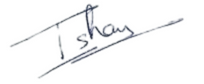
\includegraphics[scale=0.5]{Photos/Ishan_s_sign.jpeg}
\end{flushleft}
\end{figure}
Ishan Srivastava\\ 
\begin{figure}[H]
\begin{flushleft}
  
\includegraphics[scale=0.1]{Photos/Janhavi_p_sign.jpeg}
\end{flushleft}
\end{figure}
Janhavi Panambor\\
\end{raggedright}

% Names of Group Members with Signature\\  \vspace{0.5 cm}

\noindent Place : Pune \\
Date : 17-12-2021




\cleardoublepage \addcontentsline{toc}{chapter}{Abstract}
\begin{center}
{\huge \bf Abstract}
\end{center}
\vspace{20mm}
%\hspace{0.5 cm} 

Brain tumours, in medical terms are the intentional or unintentional growth of mass cells which hamper the conventional functioning of the shape of brain. For correct diagnosis and efficient treatment planning, it is necessary to detect the brain tumour in the early stages. The tumour within the brain is one of the most dangerous diseases and might be diagnosed easily and reliably with the assistance of detection of the tumour using automated techniques on MRI Images. Positron Emission Tomography, Cerebral Arteriogram, spinal tap, Molecular testing are used for tumour detection. Digital image processing plays an important role in the analysis of medical images. Segmentation of tumours involves the separation of abnormal brain tissues from normal tissues of the brain. Over few past years, various researchers have proposed semi and fully automatic methods for the detection and segmentation of Brain tumours. The motivation behind this project is to detect neoplasm and supply better treatment for the suffering. The objectives for the project are to develop an end-product (Web Application) that can be installed at hospitals. To facilitate this a detection model is developed that may accurately predict if an uploaded MRI scan of brain shows it is affected by tumour or not. To implement the project a Convolutional Neural Network(CNN) was used to define the model. Transfer Learning is implemented in order to efficiently train the model. The data-set used is split into 3 sets which are train, test and validation, in the ratio 80:10:10. The model is meant to be trained for 12 epochs. Callbacks also have been given to automate the model save process. The test accuracy of 97\% is achieved. This trained model will be connected with an online Application via API. Within the proposed Web App the user is having access to four routes which is welcome page and this contains information about the system, second route is information and awareness about the brain tumour in medical terms, third is detection page, where the trained model is deployed. The user is able to provide an input image, MRI images in our case, and last route is the team information. Images which are fed to the model route will be processed by the developed convolutional neural network which is able to then confirm if a tumour is present or not and intimidate the user for the same through an output Display. The advantage of using this system is that it will automate the detection process, and ease the workload of the hospital staff. However for the advantage to become a reality, careful selection of accurate data is needed, else there is a chance of false results.\\ 

{\bf{Keywords:}}\\ Brain Tumour Detection, Medical Image Processing, Brain tumour, MRI, CNN, Web Application, Case History 

\newpage
\cleardoublepage \addcontentsline{toc}{chapter}{Contents}
\tableofcontents
\cleardoublepage \addcontentsline{toc}{chapter}{List of Figures}
\listoffigures
\cleardoublepage \addcontentsline{toc}{chapter}{List of Tables}
\listoftables
\cleardoublepage \addcontentsline{toc}{chapter}{List of Abbrevations}
%% It is just an empty TeX file.
%% Write your code here.
\begin{center}
{\bf \Large LIST OF ABBREVIATIONS}
\end{center}
%lease add the following required packages to your document preamble:
% \usepackage{graphicx}
\begin{table}[H]
\centering
%\resizebox{\textwidth}{!}{%
\begin{tabular}{ll}
AI & Artificial Intelligence\\
ML & Machine Learning\\
DL & Deep Learning\\
CNN & Convolutional Neural Network\\
ANN & Artificial Neural Network\\
MRI & Magnetic Resonance Imaging\\
PET & Positron Emission Tomography\\
CT & Computer Tomography\\
SPECT & Single-Photon Emission Computed Tomography\\
UI & User Interface\\
SOM & Self Organizing Algorithm\\
LE & Laplacian Eigenmaps\\ 
ICA & Independent Component Analysis\\
AHC & Agglomerative Hierarchical Clustering\\
DWAE & Deep Wavelet AutoEncoder model\\
\end{tabular}%
%}
\end{table}
\cleardoublepage
\pagestyle{plain}
\pagenumbering{arabic}

\chapter{Introduction}
Initiating the chapter, Artificial Intelligence and its allied areas are witnessing the rapid growth and advancements for removing the barrier between humans and machines for a better world and future ahead. This deals with the biomedical domain of technology very specifically with the brain tumours and their detection with traditional ways and a brief light to modern future approaches with the use of technology. The introduction starts with an overview of the problem statement which is an early-stage detection of brain tumours. Traditional approaches of detecting and factors associated with it. Image processing is the heart of the detection through Deep Learning and Machine learning models. The detection is done via deep learning methods comprising particular algorithms. Convolutional Neural Network is the heart of image analysis using machine learning or deep learning models which offers ease of analysis with good efficiency. Followed in the next section shows the significance of Computer Vision that can be helpful for image analysis. 
\section{Overvew of the detection system}

{Computer vision and image processing are a few of the most significant domains in upcoming technical advancements of the world. The main objective of computer vision and Image processing is to enable machines and devices to view and capture the world in the way humans see it. It is the entire process involving object detection, classification and analysing the results. Image processing has majorly two parts involved in the entire process. Pre-processing is the first step in image processing which consists of operations such as image enhancement, resizing, adjusting images. Post Processing comes as the second part in the process which has special modifications as per the needs - highlighting the segmented areas, removing noise, applying texts to the area needed. Thus, any image dataset which consists of similar fields can be processed and modified for particular needs to tackle the problems.}\\

{Artificial Intelligence and its effects have seen an exponential rise in advancements of the world through automation and smart technologies. Artificial Intelligence alongside machine learning and deep learning techniques have been embedded into almost every aspect of life. With the advent of Smart tools and systems using AI-ML-DL, both developers and consumers have been benefited in terms of better business deals and revenue generation. It is highly significant to today's highly sophisticated technical era of the world to make better decisions using such advanced systems and implement - integrate them into their real-life as per their needs.}\\

{In this paper, a system for the early-stage detection of brain tumours is proposed. As the human brain is the most important body organ and its improper working or disease can lead to mortality death with tumours. Hence a system based on image segmentation and the deep learning algorithm is proposed for early-stage detection of these tumours. }\\

{Brain tumours or neoplasm are basically the growth or mass of abnormal cells which grow inside the Brain. There has been an unprecedented growth in the number of humans diagnosed with Brain Tumours. There are two prominent types of brain Tumours one is benign ( non - cancerous ) and another one is Malignant ( cancerous ). There are various methodologies to detect them and validate the same with tissue tests. Traditional approaches to detecting brain tumours and treating them cost a lot of money and time, which is in most cases not suitable for middle-class men and dependents. All these factors contribute as disadvantages and thus it is beneficial to bring technology into consideration and use existing infrastructure as an algorithm so that we can detect a tumour at an early stage and save a lot of money and consume less time. Adding to this, the mortality rate can be reduced by early detection of tumours. Humans are living in an age where health becomes a very crucial factor in order to maintain and then survive thus, having such a biomedical system can be highly efficient in terms of money and time.}\\

{The solution is an easy and simple brain tumour detection system that uses CNN - convolutional neural network algorithm and feeds on image input by the user which then segments the image and applies image processing and highlights if it detects brain tumour with proper highlighting.}\\

{The motivation behind selecting the particular project is the statistics observed till now. Brain Tumour incidence has increased more than 10\% over the past 20 years(paper 8). Such an increase in incidence puts higher pressure on the existing medical facilities. Thereby a simple solution is proposed that can help in solving the issue.}\\

{What our system does is it uses a end product ( web app ) which will have inputs as MRI scanned images of brain, it will perform digital image processing on the input image and will undergo CNN algorithm process. This involves validation and comparison with our trained model and based on its learning, it will classify whether it a tumour or not. If tumour, it will highlight the area affected inside the brain. Since brain tumour varies on the location it is affected, we can have a long run effect insight also from the same output. These insigts and reports can be stored on the same web application and cab be used further to compare the change in earlier records of the same patient also. }\\

{Overall, in a nutshell, early information on the brain tumour and how well it can be diagnosed can be obtained.}\\

The report is divided into 6 chapters. Chapter 1 deals with the basic introduction of the project. The chapter also deals with what a brain tumour actually is. Furthermore, problem motivation for the project and an overview of the project system is provided. Chapter 2 deals with the Literature Survey conducted. The literature survey highlights papers that give an insight into different algorithms, techniques and processing that can be used to detect brain tumours. Chapter 3 deals with Problem statements, Outcomes, Requirement Analysis, Impact Analysis and Limitations. A brief has also been given on Professional Ethics to be followed during the implementation of the project. Chapter 4 deals with the actual project implementation. Here a summary as to what resources are required actually, the basic block diagram have been discussed. Furthermore, the Detection Model and Webapp have been discussed in brief with flowcharts and algorithms. A model summary used has also been provided. At the end images of the proposed layout have also been attached for ease of understanding. Chapter 5 deals with the results obtained from the detection model, as well as results from the data augmentation. Chapter 6 deals with the future scope and conclusion.\\
%

\chapter{Literature Survey}

1) Authors in \cite{ref1} develop a system to detect brain tumor using Convolutional Neural Network(CNN). The paper mentions the dataset used for training. The same data has been used for the development of the system proposed in this project. The authors mention various other steps implemented which include image augmentation, pre processing, segmentation of the skull, which can be implemented for better training of the model. The authors have used a custom architecture of CNN which provides an efficiency of 95.3\% on test images. The model used by the authors is as follows : 
\begin{figure}[H]
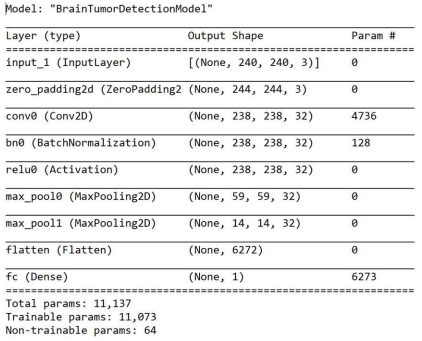
\includegraphics[scale=1]{Photos/paper1_model.PNG}
\caption{Paper 1 Model Summary} \label{fig:ishan}
\end{figure}

2) Authors in \cite{ref2} , \cite{ref3} and \cite{ref5} provides an insight into various symptoms, causes and statistics of brain tumor. This data will be used into the information module of the web application.\\ 

3) Authors in \cite{ref4} provide a survey on major deep learning systems implemented to do various types of brain tumor analysis. This survey gives an insight into the existing detection models. The paper further gives an insight into datasets, techniques into consideration as well as the evaluation of each particular paper considered into the survey.\\

4) Authors in \cite{ref5} use image segmentation as the base technique for detection purpose. The authors use a clustering based approach using Self Organizing Map (SOM) algorithm. The detection works in two phases, the first being image acquisition and pre processing. The second phase is image segmentation which basically segments principle tissue structures in the input images. The authors propose a new MR image segmentation method based on fuzzy C-Means clustering algorithm for the Segmentation which is unsupervised. \\

5) Authors in \cite{ref6} compare nonlinearity reduction with linear method. The authors experiment to check if the non linear method provide better results (unsupervised classification) of MRS brain tumor data. Data reduction is performed using Laplacian eigenmaps (LE) or independent component analysis(ICA). This was then followed by k-means clustering or agglomerative hierarchical clustering (AHC) for unsupervised learning to assess tumor grade and for tissue type segmentation of MRSI data. Based on the results obtained LE method is promising for unsupervised clustering to separate brain and tumor tissue with automated color-coding for visualization of 1 H MRSI data after cluster analysis.\\

6) Authors in \cite{ref7} conduct a survey on different segmentation techniques. The paper provides different papers, their datasets, and various parameter information that gives a brief insight into different algorithms that can be implemented to detect brain tumor. The survey is divided into the following categories: Thresholding techniques, Region growing techniques, Edge based techniques, Clustering techniques, Watershed technique, and Deformable model-based techniques.\\

7) Authors in \cite{ref8} focuses on using image segmentation for brain tumour detection. From the paper it can be inferred that Magnetic Resonance Imaging (MRI) scans are the best medical scan for the training and detection of brain tumour. A deep insight is given into the different parameters associated with image enhancement using different filters and techniques. Furthermore insights are also provided into segmentation techniques.

8) Authors in \cite{ref9} proposed a deep wavelet autoencoder model named "DWAE Model". A high pass filter is used to show the heterogeneity of MRI images. After preprocessing is performed,  the DWAE Model analyzes the pixel pattern of the input scan, and classifies the tumor accordingly. The test results show that the model achieves an accuracy of 99.3\% with a validation loss of 0.1\%.
\chapter{Proposed Methodology}
\section{Problem Statement}
To detect brain tumour using Deep Learning algorithms and implement the same into a web application that will act as an end product. The system being developed aims to facilitate early detection of tumour so as to reduce mortality rates. 
\subsection{Objective}
Objectives of the project are to reduce human intervention using automation. To implement the automation part a web application will be used. It will integrate a detection model which will automatically which type of tumour is present, based on the inference it obtains. Another objective is to reduce medical treatment costs, by early detection of tumour.

\subsection{Outcome}
Outcomes of this project are as follows:
A model system, which analyses the presence of brain tumour, after scanning. It traces the brain tumour present in the MRI Scan, and identifies the presence of Brain Tumour. The Brain Tumour is identified through the automation, which is trained, to identify the presence or absence through simple algorithm. After implementing the specific methodology, the model system is able to accurately detect brain tumour and then provide further insights for the same.

\section{Basic Block Diagram}
The web application will use the trained model for detection of brain tumour. This detection system works on pre trained models that are able to analyze the input images provided by the end users. Once the system has input images, it performs pre-processing operations on it. Pre-processing is the name for operations on images at the lowest level of abstraction whose aim is an improvement of the image data that suppress undesired distortions or enhances some image features important for further processing. Some of the steps in the Pre-processing include converting the image to grayscale, detecting the skull and brain part in the MRI image and so on. Once the Pre-processing is done, the system determines whether the input MRI image contains any tumour or not. Based on the results obtained from the detection, the system performs post processing. Post processing includes operations such as enhancement of the image. This segment is the processed result image. As part of output result, the system will provide a message on the web application regarding the tumour inference, as well as suggestions for treatment.
\begin{figure}[H]
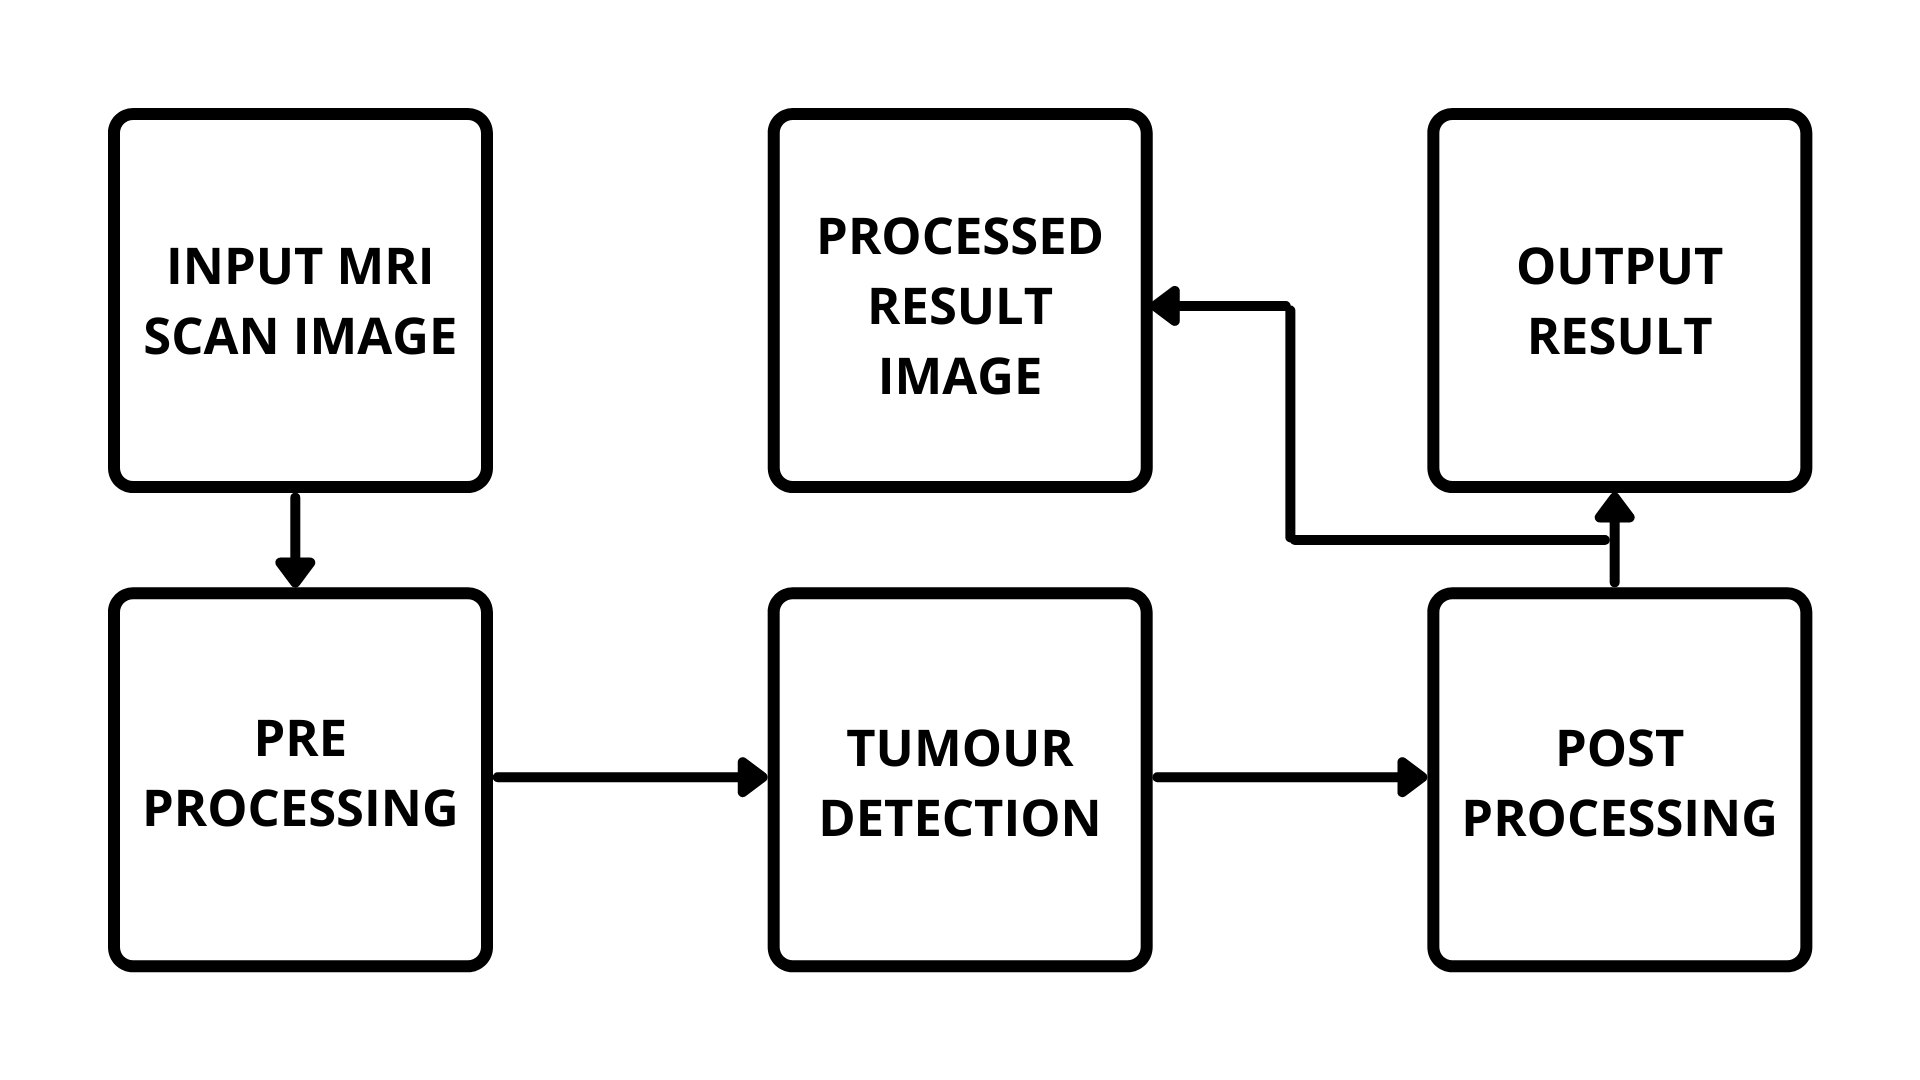
\includegraphics[scale=0.2]{Photos/blockdiagram.png}
\caption{Block Diagram} \label{fig:ishan}
\end{figure}
%%%%%%%%%%%%%%%%%%%%%%%%%%%%%%%%%%%%%%%%%%%%%%%%%%%%%%%%%%%%%
\section{Requirement analysis}
\subsection{Hardware Requirement}
The only hardware requirement for the project which has been observed till now are as follows:
\begin{itemize}
    \item An End device such as Laptop/PC(Both to train the model and for developing and accessing the web application)
\end{itemize}
%\subsection{Software Requirement}
%Explain about the appropriate Software Requirement with proper reasoning. (This is mandatory section)
\subsection{Modern Engineering Tools and Software Requirement}
{\textbf{a) Open Source Libraries / Softwares / Tools Requirement:}}
\begin{itemize}
    \item A python development environment : Any python environment is needed to train the model which will inturn detect the tumour. For our particular project we have opted for Kaggle Cloud Editor. For the mentioned below reasons:
        \begin{itemize}
            \item Higher computational power.
            \item Ease of importing data from datasets.
            \item Version control of code.
        \end{itemize}
        \begin{figure}[H]
        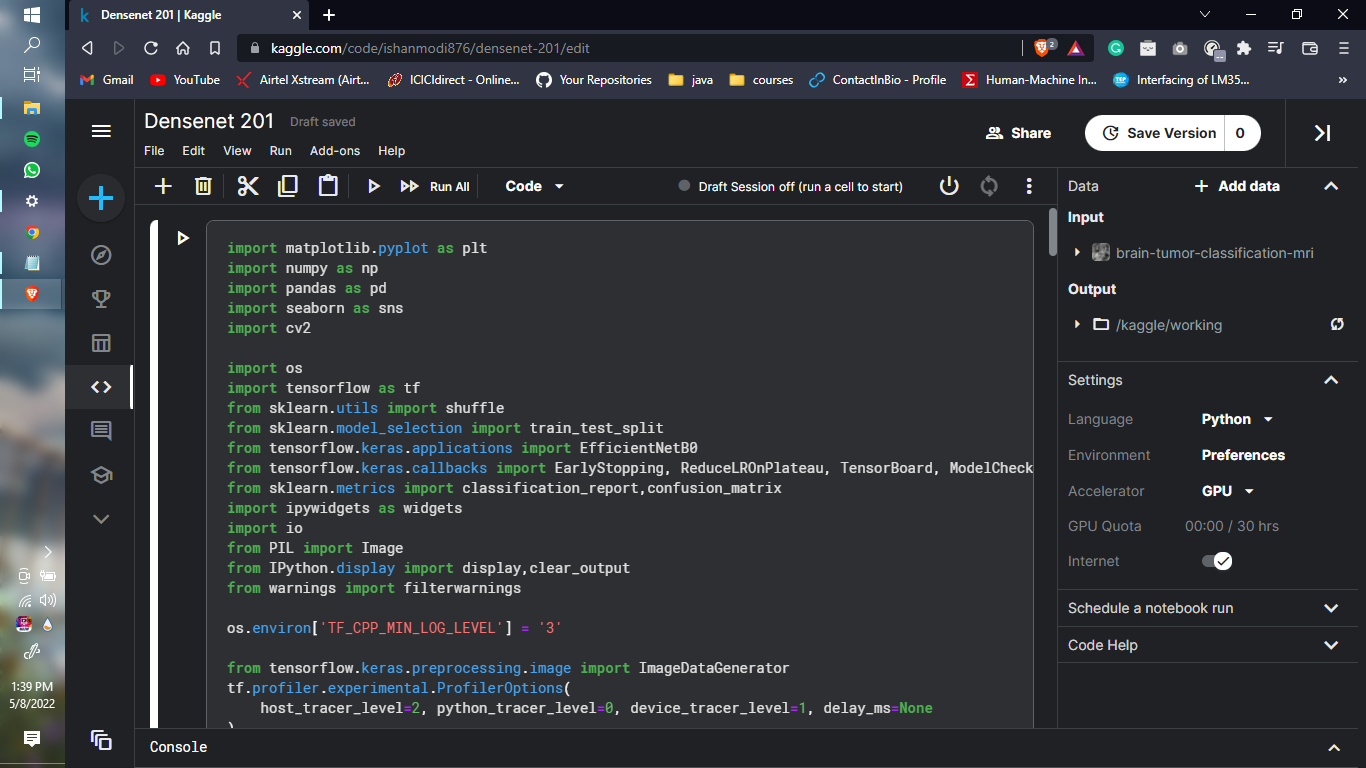
\includegraphics[scale=0.3]{Photos/Kaggle_Editor2.png}
        \caption{Kaggle Editor} \label{fig:ishan}
        \end{figure}
    \item Python Libraries : To implement the project, various libraries are needed to perform the required functionality that we desire. We need Python libraries both for the training of the model as well as to develop the web application. The libraries which have been used until now are as follows:
        % Please add the following required packages to your document preamble:
        % \usepackage{graphicx}
        % \usepackage[table,xcdraw]{xcolor}
        % If you use beamer only pass "xcolor=table" option, i.e. \documentclass[xcolor=table]{beamer}
        % Please add the following required packages to your document preamble:
% \usepackage{graphicx}
% \usepackage[table,xcdraw]{xcolor}
% If you use beamer only pass "xcolor=table" option, i.e. \documentclass[xcolor=table]{beamer}
        \begin{table}[h!]
        \caption{List of Python libraries used:}
        \label{tab:table1}
        \resizebox{\textwidth}{!}{%
        \begin{tabular}{|c|c|c|}
        \hline
        \rowcolor[HTML]{CBCEFB}  
\textbf{Library} & \textbf{Function}                                                                                                                                                                    & \textbf{Version(if applicable)} \\ \hline
OS               & \begin{tabular}[c]{@{}c@{}}Creating and removing a directory(folder),\\ fetching its contents, changing and identifying the current director.\end{tabular}                           & N/A                             \\ \hline
Keras            & \begin{tabular}[c]{@{}c@{}}Provide python interface for Neural Networks.\\ Also acts as an interface for Tensorflow Library.\\ Also used to define layers to the model.\end{tabular} & 2.6.0                           \\ \hline
Tensorflow       & \begin{tabular}[c]{@{}c@{}}Training and inference of deep neural networks.\\ Also used for establishing callbacks\end{tabular}                                                       & 2.6.1                           \\ \hline
Numpy            & Library for working with multi-dimensional arrays.                                                                                                                                   & 1.21.4                          \\ \hline
Pandas           & Data Manipulation and Analysis                                                                                                                                                       & 1.3.5                           \\ \hline
Matplotlib       & Data visualization and graphical plotting library                                                                                                                                    & 3.5.1                           \\ \hline
Sklearn          & \begin{tabular}[c]{@{}c@{}}Machine Learning library of Python.\\ Features various algorithms such as random forests, K-neighbours etc.\end{tabular}                                  & 0.23.2                          \\ \hline
Time             & Representing time in code                                                                                                                                                            & 3.7.0                           \\ \hline
Imutils          & Basic Image Processing                                                                                                                                                               & 0.5.4                           \\ \hline
Cv2              & Image Processing and computer vision                                                                                                                                                 & 4.5.4.60                        \\ \hline
Shutil           & Copy and Removal of files                                                                                                                                                            & 3.10.1                          \\ \hline
Seaborn          & Python Data Visualization library based on Matplotlib                                                                                                                                & 0.11.2                          \\ \hline
Ipywidgets       & Interactive HTML widgets for Jupyter and Ipython Console                                                                                                                             & 8.00rc0                         \\ \hline
\end{tabular}%
}
\end{table}
    \item LaTeX Editor : LaTeX is a high-quality typesetting system; it includes features designed for the production of technical and scientific documentation. LaTeX being a language system needs a system software to support it's functionality. For the project Papeeria has been used to write the project report.
    \item  \href{https://www.analyticsvidhya.com/blog/2021/06/build-web-app-instantly-for-machine-learning-using-streamlit/}{Streamlit Framework} : Streamlit is an open-source python framework for building web apps for Machine Learning and Data Science. We can instantly develop web apps and deploy them easily using Streamlit. Streamlit allows you to write an app the same way you write a python code. Streamlit makes it seamless to work on the interactive loop of coding and viewing results in the web app.
    %\begin{figure}[H]
    %    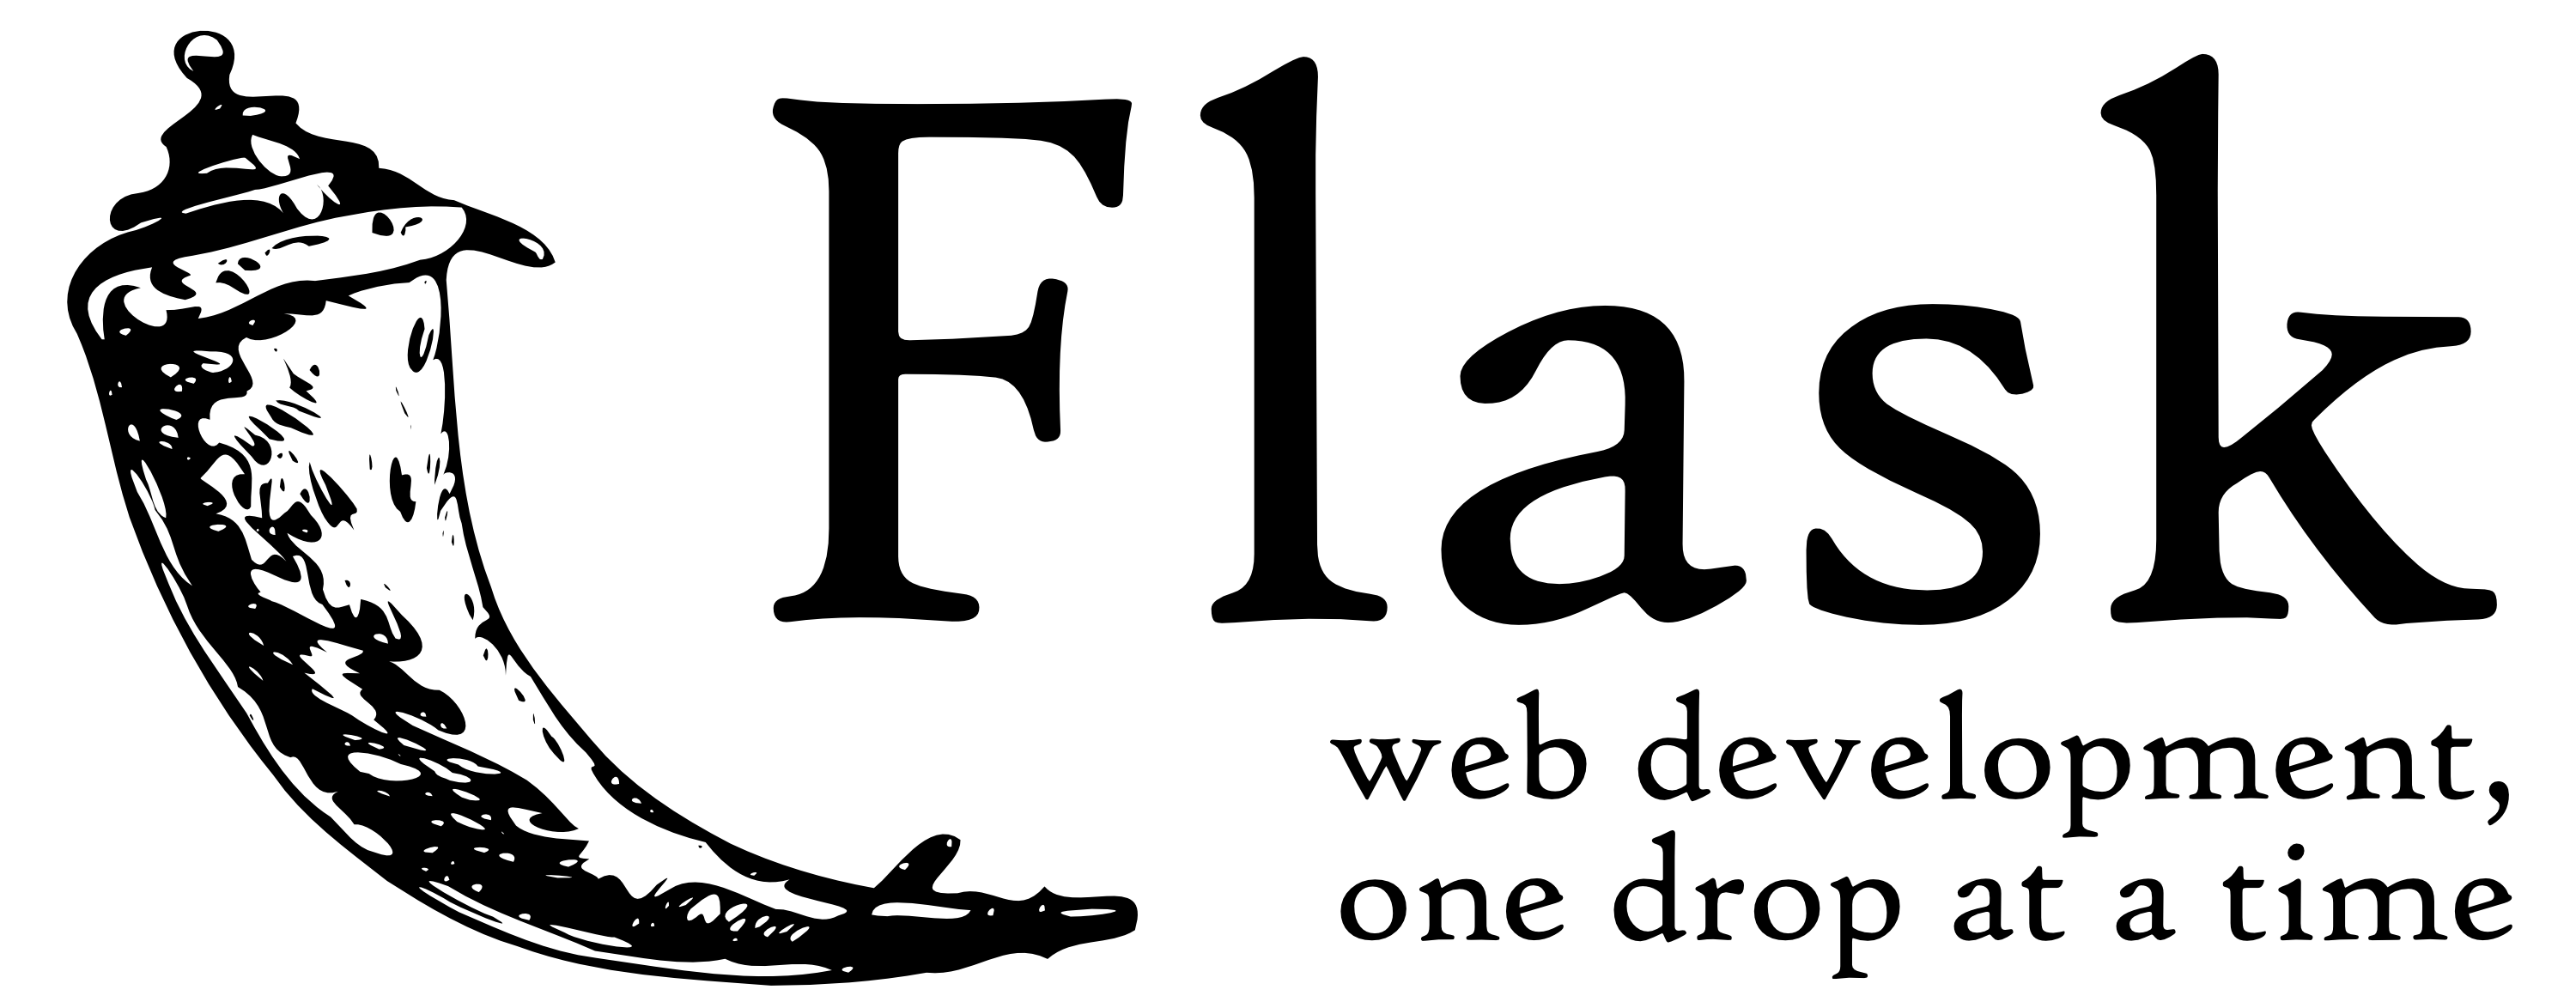
\includegraphics[scale=0.001]{Photos/flask.png}
    %    \caption{Flask Web Framework} \label{fig:flask}
    %    \end{figure}
\end{itemize}
{\textbf{b) Proprietary Softwares / Libraries / Cloud Requirement:}}\\ 
Proprietary Software include both OS and software applications contained within it. The Proprietary Softwares which have been used in the duration of Phase-1 of the project are as follows:
\begin{itemize}
    \item Windows OS : Windows OS is the base Operating System, which has been used to develop the code base as well as to do the paper work.
    \item Microsoft Powerpoint : Microsoft Powerpoint is a proprietary software by Microsoft which has been used to make the presentations for the project as well as develop a proposed UI of the web application.
\end{itemize}
\subsection{Resources Requirement}
    \begin{itemize}
    \item Datasets : To train the model efficiently datasets are needed which contain the data(MRI scan images in our case). This data is fed to the model which then trains it to detect whether the MRI scan is tumorous or non-tumorous and further classify the tumorous images into 3 categories : Meningioma, Pituitary and Glioma. For the project one dataset has been utilized. The dataset contains 4 subfolders each containing images under four labels as follows : Pituitary, Meningioma, Glioma and Non-Tumorous . The Dataset is as follows:
        \begin{itemize}
            \item \href{https://www.kaggle.com/datasets/sartajbhuvaji/brain-tumor-classification-mri}{Brain Tumor Classification (MRI)} : \\
                Table (\ref{tab:Dataset}) gives an insight into the contents within the dataset: 
                % Please add the following required packages to your document preamble:
% \usepackage{multirow}
% \usepackage{graphicx}
% \usepackage[table,xcdraw]{xcolor}
% If you use beamer only pass "xcolor=table" option, i.e. \documentclass[xcolor=table]{beamer}
\begin{table}[h!]
                \caption{Contents of Brain MRI Images for Brain Tumor Detection Dataset}
                \label{tab:Dataset}
\begin{tabular}{c|c|c|}
\cline{2-3}
\multicolumn{1}{l|}{}                                                                                                        & \cellcolor[HTML]{CBCEFB}\textbf{Data Label} & \cellcolor[HTML]{CBCEFB}\textbf{No. Of Images} \\ \hline
\multicolumn{1}{|c|}{\cellcolor[HTML]{CBCEFB}}                                                                               & Glioma                                      & 100                                            \\ \cline{2-3} 
\multicolumn{1}{|c|}{\cellcolor[HTML]{CBCEFB}}                                                                               & Meningioma                                  & 115                                            \\ \cline{2-3} 
\multicolumn{1}{|c|}{\cellcolor[HTML]{CBCEFB}}                                                                               & No Tumour                                   & 105                                            \\ \cline{2-3} 
\multicolumn{1}{|c|}{\multirow{-4}{*}{\cellcolor[HTML]{CBCEFB}\textbf{\begin{tabular}[c]{@{}c@{}}Test\\ Set\end{tabular}}}}  & Pituitary                                   & 74                                             \\ \hline
\multicolumn{1}{|c|}{\cellcolor[HTML]{CBCEFB}}                                                                               & Glioma                                      & 826                                            \\ \cline{2-3} 
\multicolumn{1}{|c|}{\cellcolor[HTML]{CBCEFB}}                                                                               & Meningioma                                  & 822                                            \\ \cline{2-3} 
\multicolumn{1}{|c|}{\cellcolor[HTML]{CBCEFB}}                                                                               & No Tumour                                   & 395                                            \\ \cline{2-3} 
\multicolumn{1}{|c|}{\multirow{-4}{*}{\cellcolor[HTML]{CBCEFB}\textbf{\begin{tabular}[c]{@{}c@{}}Train\\ Set\end{tabular}}}} & Pituitary                                   & 827                                            \\ \hline
\end{tabular}%
\end{table} \\
Figure (\ref{fig:data_sample}) plots some sample images from the dataset.
\begin{figure}[H]
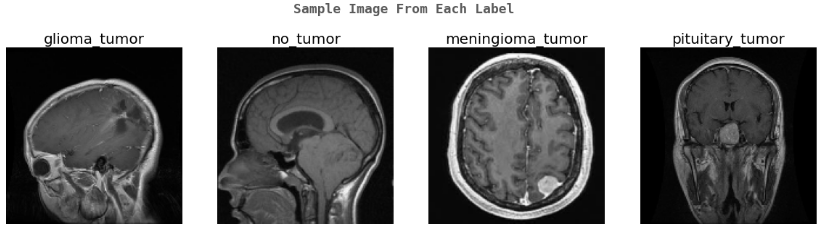
\includegraphics[scale=0.55]{Photos/dataset_sample1.PNG}
\caption{Sample Images from Dataset} \label{fig:data_sample}
\end{figure}
        \end{itemize}
        \item Graphical Images : Graphical Images are needed for the Web Application. This is purely a resource requirement for an end user product and is not needed for any core functionality of the system.
    \end{itemize}


\section{Impact analysis}
\subsection{Impact of project on society}
{\textbf{Positive Impact of project on society:}} 
\begin{itemize}
    \item Early detection of tumour can reduce the cost required to treat the tumour.
    \item Early detection can overall improve the lifespan of humans.
\end{itemize}
{\textbf{Negative Impact of project on society:}}
\begin{itemize}
    \item It has a risk of errors and wrong detection due to less training.
    \item It has a risk of not detecting Initial stages of tumour due to small size.
\end{itemize}
\subsection{Impact of project on environment }
{\textbf{Positive Impact of project on environment: }}
\begin{itemize}
    \item Less Bio Medical waste is generated due to early detection and treatment.
\end{itemize} 
{\textbf{Negative Impact of project on environment: }}
\begin{itemize}
    \item Bio Medical waste generated during treatment after the detection of tumour is done through this system, if not treated properly can pose environmental risks.
\end{itemize}

\section{Limitations}
\begin{itemize}
    \item Limited detection due to less datasets being used in training.
    \item Accuracy of Dataset is an important factor. Unverified datasets can lead to false results.
    \item The detection model in it's base form cannot provide accurate results on MRI captured using higher tesla MRI Machines.
\end{itemize}

\section{Professional ethical practices to be followed}
\begin{itemize}
    \item Giving credits wherever due.
    \item Keeping technical guidelines in mind.
    \item Following the norms of engineering Practices.
    \item Liabality for outcome caused by one’s actions or decisions.
\end{itemize}

\chapter{Project Implementation}
Initiating the chapter, here project implementation is discussed. The resources required, flowcharts, algorithms as well as proposed layouts have been highlighted here.
\section{Requirement of Resources}
\begin{itemize}
    \item Software Requirement 
        \begin{enumerate}
            \item OS Requirement:
                \begin{itemize}
                    \item Windows 8/10(Can be used both for Training and at User End)
                    \item Linux(Only at User End)
                \end{itemize}
            \item Training of the model:
                \begin{itemize}
                    \item Python ide(Anaconda Jupyter Notebook/Jupyter Lab)
                    \item Dataset for Training
                \end{itemize} 
            \item Web Application
        \end{enumerate}
    \item Hardware Requirement
        \begin{enumerate}
            \item Basic Hardware for Training Purpose:
                \begin{itemize}
                    \item RAM : 8 GB
                    \item ROM : 2 GB
                    \item Processor : i5 Processor
                \end{itemize}
        \end{enumerate}
    \end{itemize}



%%%%%%%%%%%%%%%%%%%%%%%%%%%%%%%%%%%%%%%%%%%%%%%%%%%%%%%%%%%%%%%%%%%%%%%%%%%%%%%%%%%%%%%%%%%%%%%%%%%%%%%%%%%%%%%%%%%%%%%%%%%%%%%%%%%%%%%%%%%%%%%%%%%%%%%%%%%%%%%%%%%%%%%%%%%%%%%%%%%%%%%%%%%%%%%%%%%%%%%%%%%%%%%%%%%%%%%%%%%%%%%%%%%%%%%%%%%%%

\section{Development of the Detection model}
This section explains about the Detection model and it's training. The model developed is the backend of this project, as it handles the core function of determining whether the MRI image present has tumor or not.
\subsection{Algorithm}
Step 1 : Import the libraries.\\ 
Step 2 : Import the datasets.\\ 
Step 3 : Create the root directory to store the Final Dataset.\\ 
Step 4 : Create the sub directories to store the images based on tumor presence/absence.\\ 
Step 5 : Augment the dataset.
Step 6 : Copy tumorous images from datasets into the Yes subdirectory.\\ 
Step 7 : Copy non-tumorous images from datasets into the No subdirectory.\\
Step 8 : One Hot Encode the images.\\ 
Step 9 : Creating data list for storing image data in numpy form, path list for storing paths of all images and result list to store data of Step 7.\\ 
Step 10 : Splitting data into train, test, and validation.\\ 
Step 11 : Defining Model Layers.\\ 
Step 12 : Defining Callbacks.\\ 
Step 13 : Training the Model.\\ 
Step 14 : Plotting the accuracy and loss graphs.\\ 
Step 15 : Evaluating the Model.\\ 
Step 16 : Manually testing the model with user input.\\ 
\subsection{Flowchart}
The flowchart below describes the process as to how the detection model is developed.
\begin{figure}[H]
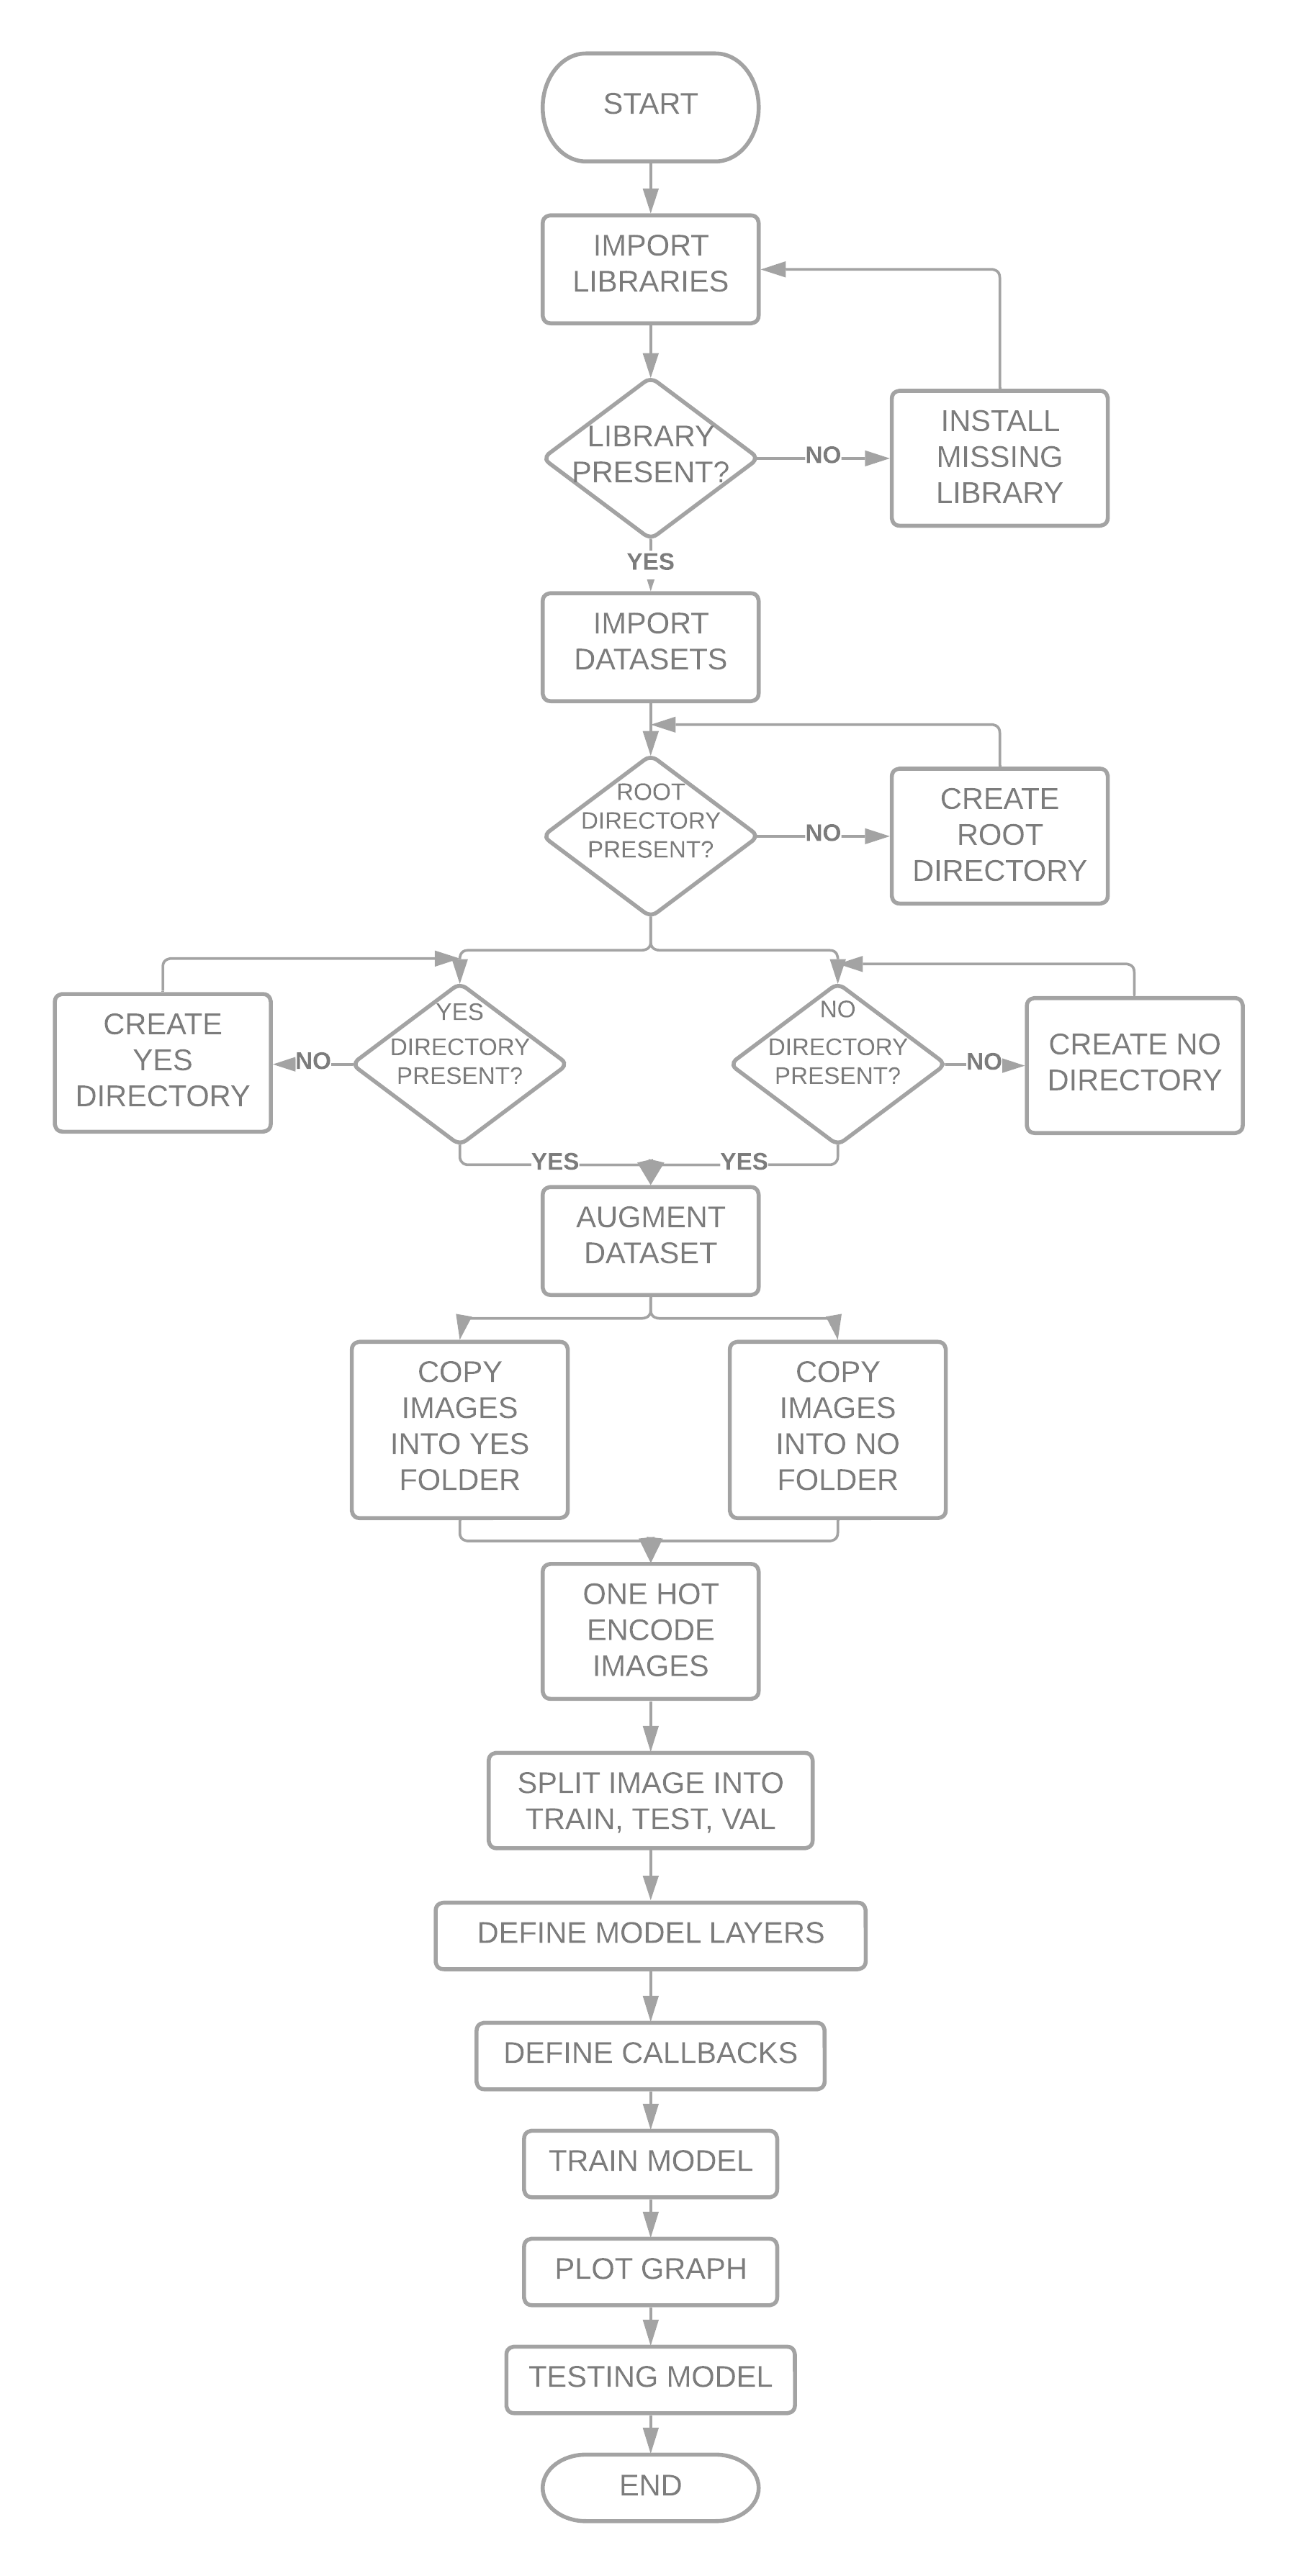
\includegraphics[scale=0.168]{Photos/model_flowchart.png}
\caption{Model Summary} \label{fig:model_flowchart}
\end{figure}
\subsection{Image Augmentation}
Image Augmentation is a technique that can be used to artificially expand the size of a training set by creating modified data from the existing one. It is a good practice to use DA if you want to prevent overfitting, or the initial dataset is too small to train on, or even if you want to squeeze better performance from your model. Figure \ref{fig:ImageAugmentation} shows an output to an image that has been augmented.
\begin{figure}[H]
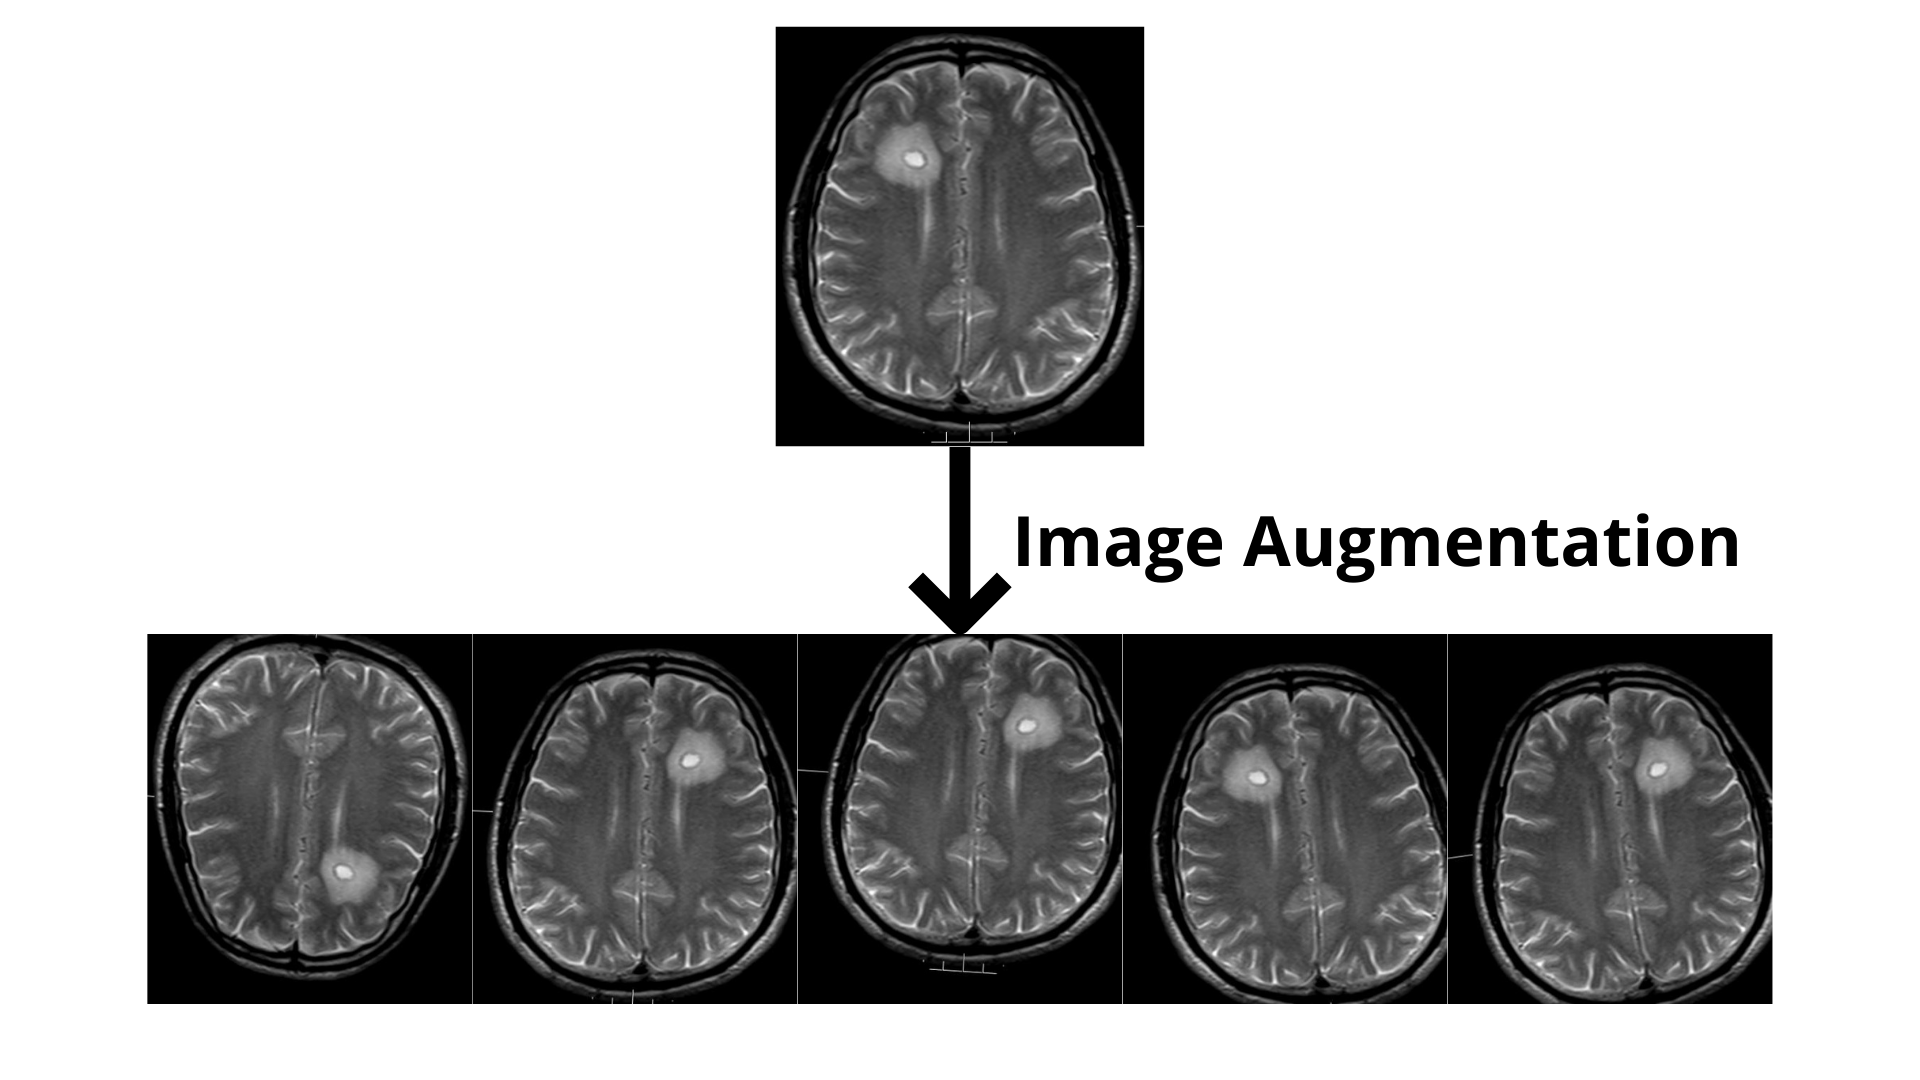
\includegraphics[scale=0.18]{Photos/ImageAugmentation.png}
\caption{Image Augmentation} \label{fig:ImageAugmentation}
\end{figure}
\subsection{Defining the Model}
The figure below summarises the model layers. A sequential model was used for the project. It is the easiest way to build a model in Keras. It allows you to build a model layer by layer. Each layer has weights that correspond to the layer the follows it.Figure \ref{fig:model_plot} shows the model architecture used in the development of the model. We use the 'add()' function to add layers to the model. To define the model following libraries must be imported, these libraries are a sub class of "keras.layers" :
\begin{itemize}
    \item Sequential : It is used to initialize the neural network.
    \item Convolution2D : This layer deals with creating a convolutional network that will deal with the MRI images.
    \item MaxPooling2D : This layer adds the pooling layers.
    \item Flatten : This layer converts the pooled feature map to a single column. This is passed to the fully connected layer.
    \item Dense : Dense layer will add this fully connected layer to the neural network.
    \item Dropout : Dropout is a technique used to prevent a model from overfitting.
    \item BatchNormalization : It is a technique for training very deep neural networks that standardizes the inputs to a layer for each mini-batch.
\end{itemize}
\begin{figure}[H]
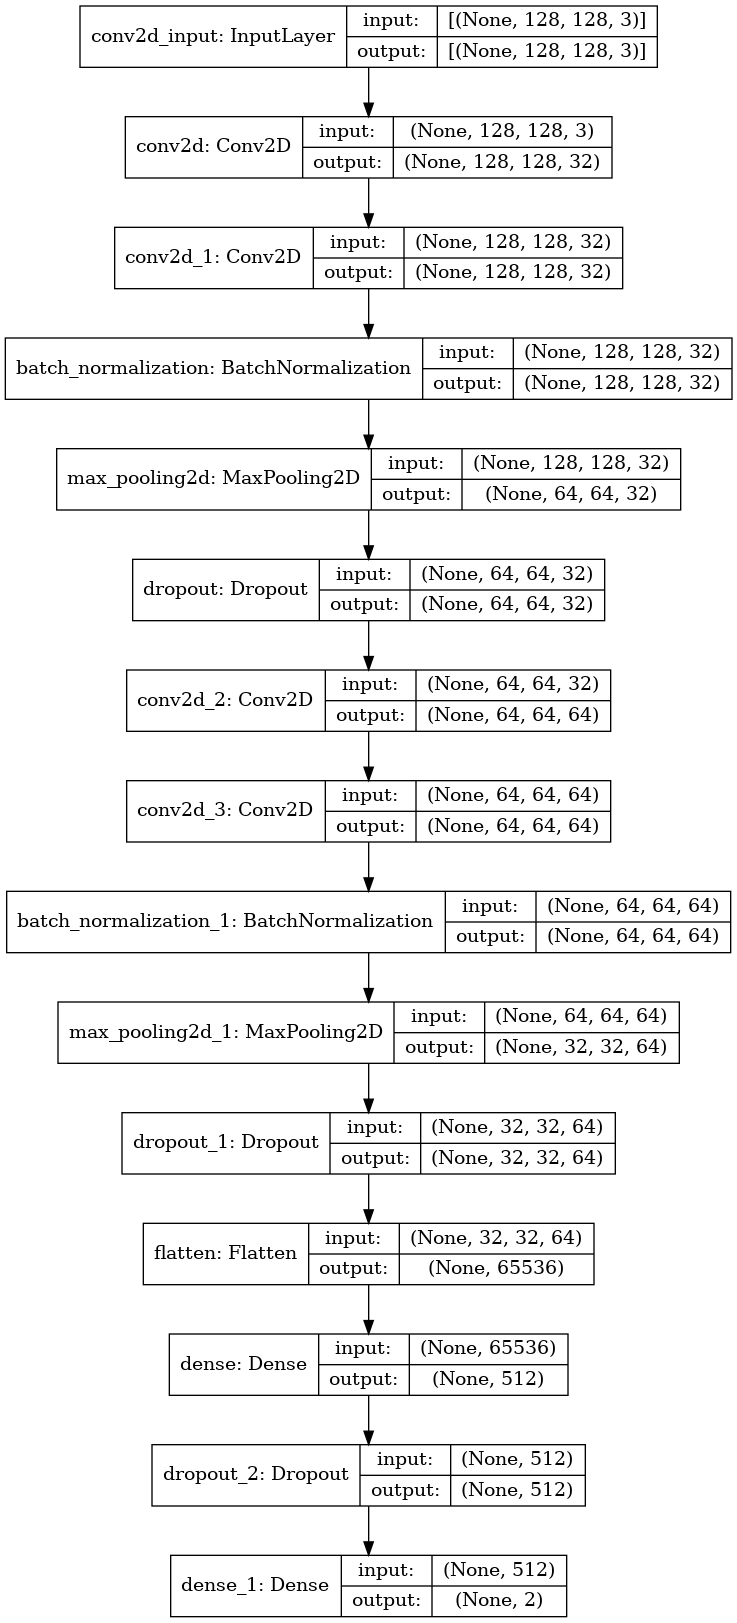
\includegraphics[scale=0.34]{Photos/model_plot.png}
\caption{Model Summary} \label{fig:model_plot}
\end{figure}

%%%%%%%%%%%%%%%%%%%%%%%%%%%%%%%%%%%%%%%%%%%%%%%%%%%%%%%%%%%%%%%%%%%%%%%%%%%%%%%%%%%%%%%%%%%%%%%%%%%%%%%%%%%%%%%%%%%%%%%%%%%%%%%%%%%%%%%%%%%%%%%%%%%%%%%%%%%%%%%%%%%%%%%%%%%%%%%%%%%%%%%%%%%%%%%%%%%%%%%%%%%%%%%%%%%%%%%%%%%%%%%%%%%%%%%%%%%%%

\section{Proposed Web Application}
This section explains about the Proposed Web Application. In this section detailed Algorithm, Flowchart and a Proposed layout is shown.
\subsection{Algorithm}
Step 1 : User is redirected to Login Page.\\
Step 2 : If the user is a New User. The Web App will redirect to Registration Page, else the user can login using his credentials. If login is unsuccessful redirect to Step 1.\\
Step 3 : After Login it will redirect to the Fact of the Day Page.\\
Step 4 : From the next page user will be able to select from 3 functionalities : Early Stage Detection, Traditional Procedures, Access History.\\
Step 5 : If user selects Early Stage Detection, webapp will redirect to the Detection Page. \\
Step 6 : User inputs Image.\\
Step 7 : System preprocesses the image.\\
Step 8 : This image is passed onto the preexisting Knowledge Base (Detection Model).\\
Step 9 : If tumor is detected, the system returns output as "Tumor Detected" and will intimate the authorities as well patient on an quick basis.\\
Step 10 : If tumor is not detected, the system returns output as "Tumor Not Detected" and will intimate the authorities as well patient on an quick basis.\\
Step 11 : If the user wants to access the menu again he can select the option and be redirected to Step 4.\\
Step 12 : If user selects Traditional Procedures, webapp will redriect to the Traditional Procedures Page.\\ 
Step 13 : If the user wants to access the menu again he can select the option and be redirected to Step 4.\\
Step 14 : If the user selects Access History, webapp will redirect to the Access History Page. \\
Step 15 : Access History Page will display the history of the patient if any. This data is directly linked to the Hospital's Database.\\
Step 16 : On clicking the About Us , Web App will redirect to the Meet Our Team Page.\\ 
Step 17 : On clicking Contact Us, Web App will redirect to Contact Us Page.\\ 
Step 18 : If user clicks Logout, Web App goes back to Step 1.\\

\subsection{Flowchart}
This is the detailed flowchart explaining the flow of the proposed webapp:
\begin{figure}[H]
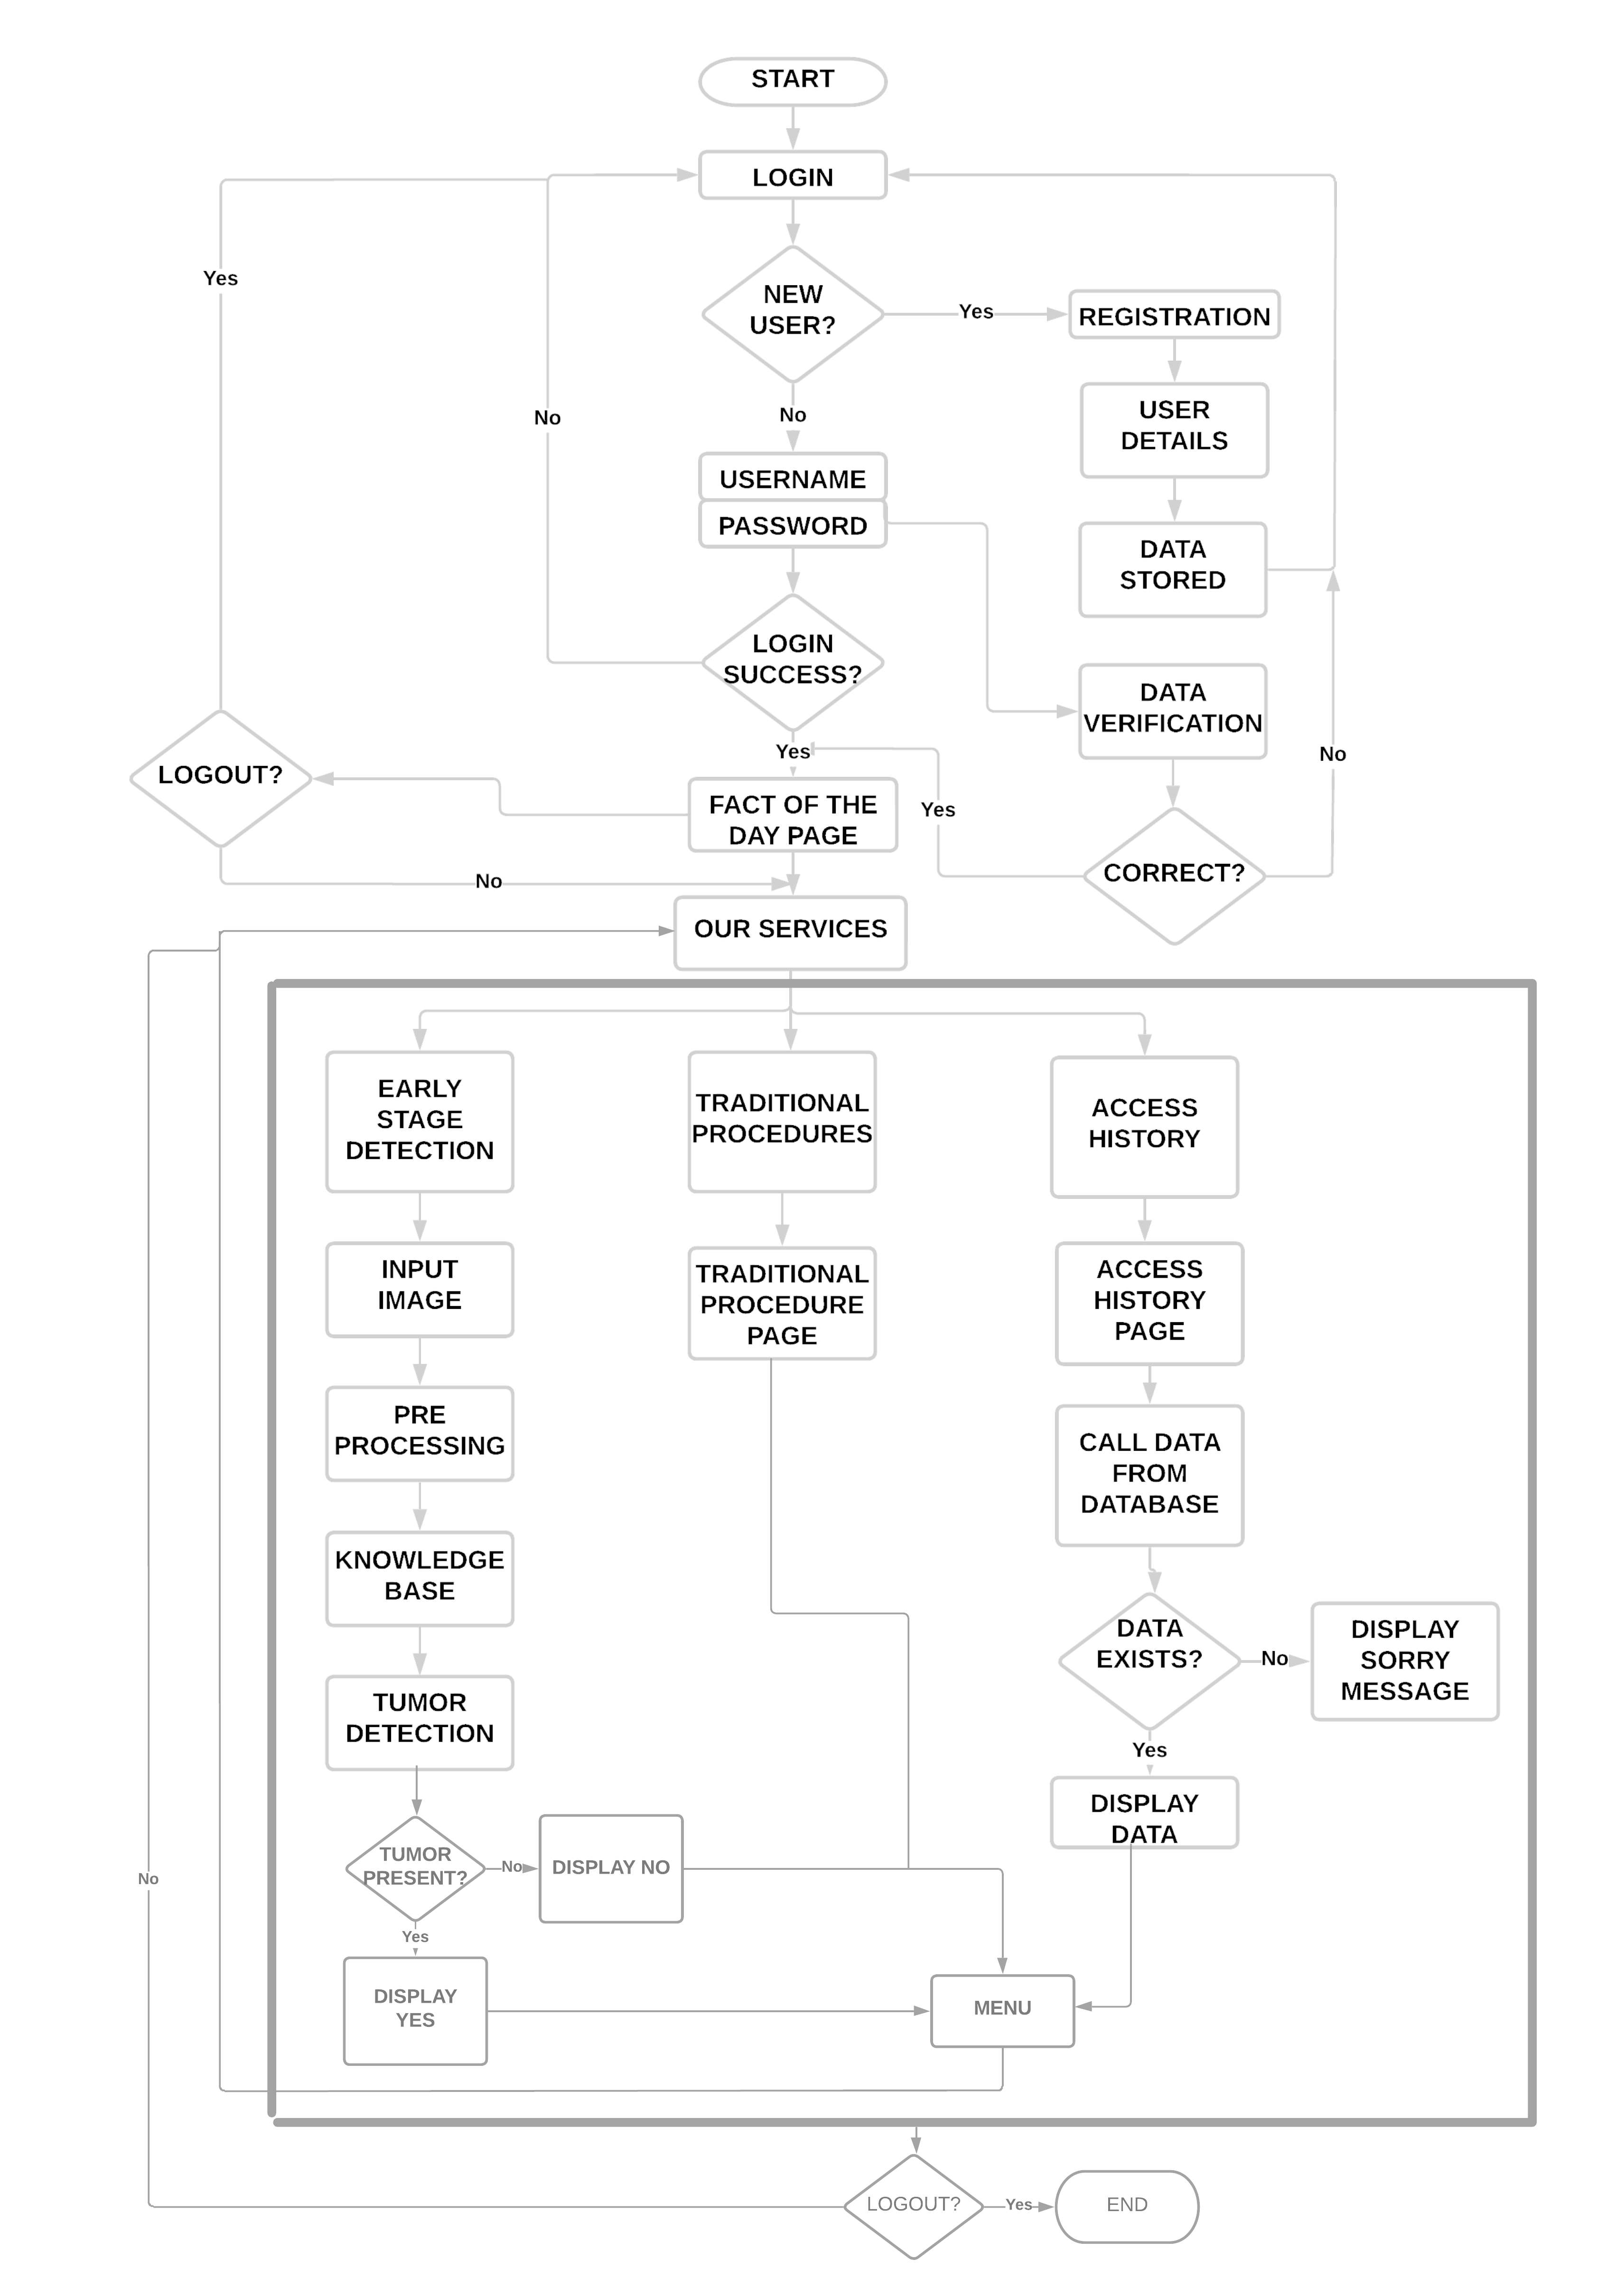
\includegraphics[scale=0.085]{Photos/webapp_flowchart.png}
\caption{Flowchart of the proposed Web Application} \label{fig:webapp_flowchart}
\end{figure}

\subsection{Proposed Web layout}
This section showcases the proposed web layout. This layout acts as a placeholder that will be used while developing the UI of the web application. While developing a web application, a layout development helps to understand the resources required, the colour schemes as well as to understand the routes of the application in consideration. \\ 
When the users will access the Web Application it will redirect to the login page(\ref{fig:webapp_1}) where both the Hospital Staff and the end user(Patient) will be able to login to access the webapp features.
\begin{figure}[H]
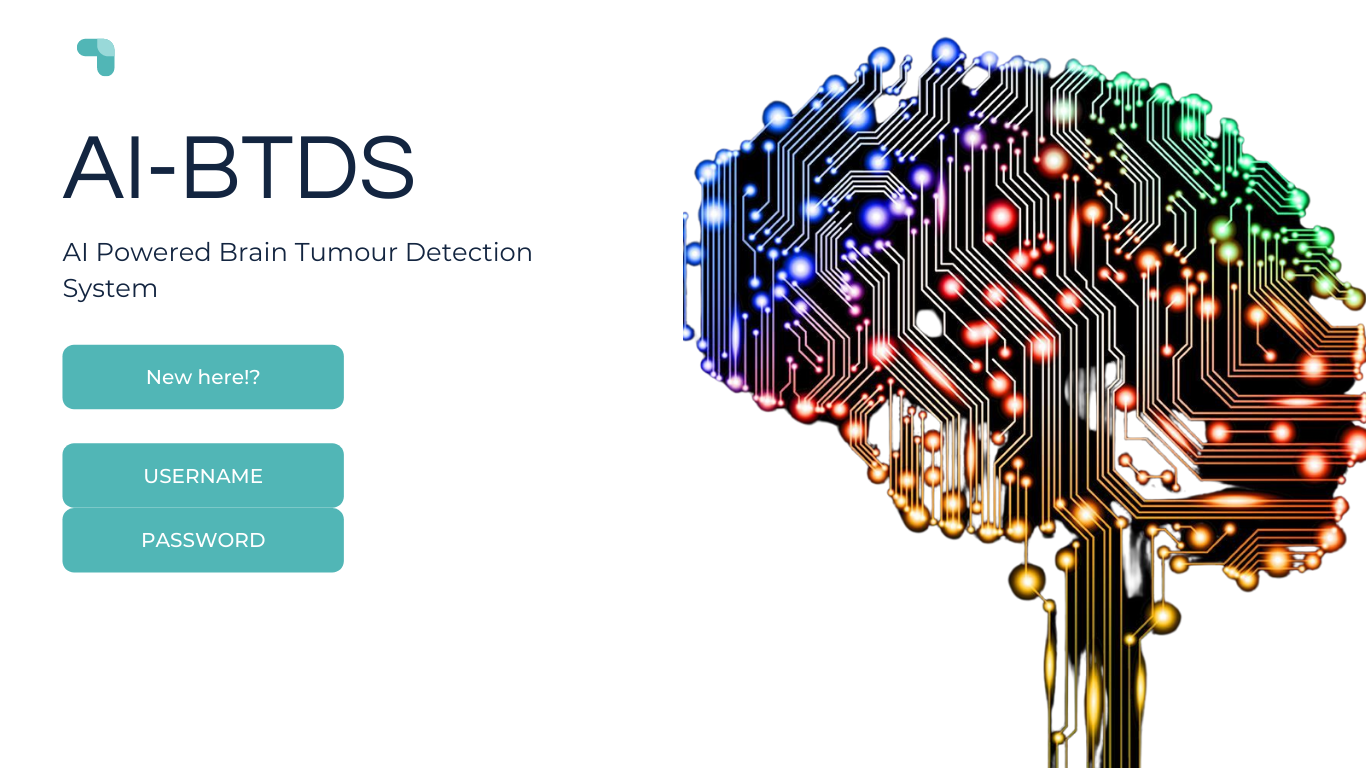
\includegraphics[scale=0.45]{Photos/webapp_1.png}
\caption{Login Page} \label{fig:webapp_1}
\end{figure}
The next figure is the Facts Page (\ref{fig:webapp_2}). The web application will be having an additional functionality that will provide information on brain tumor as well so as to increase general awareness. This will be done using a random function generator that will display a new fact based on two factors, whether the user reloads the web page or based on time.
\begin{figure}[H]
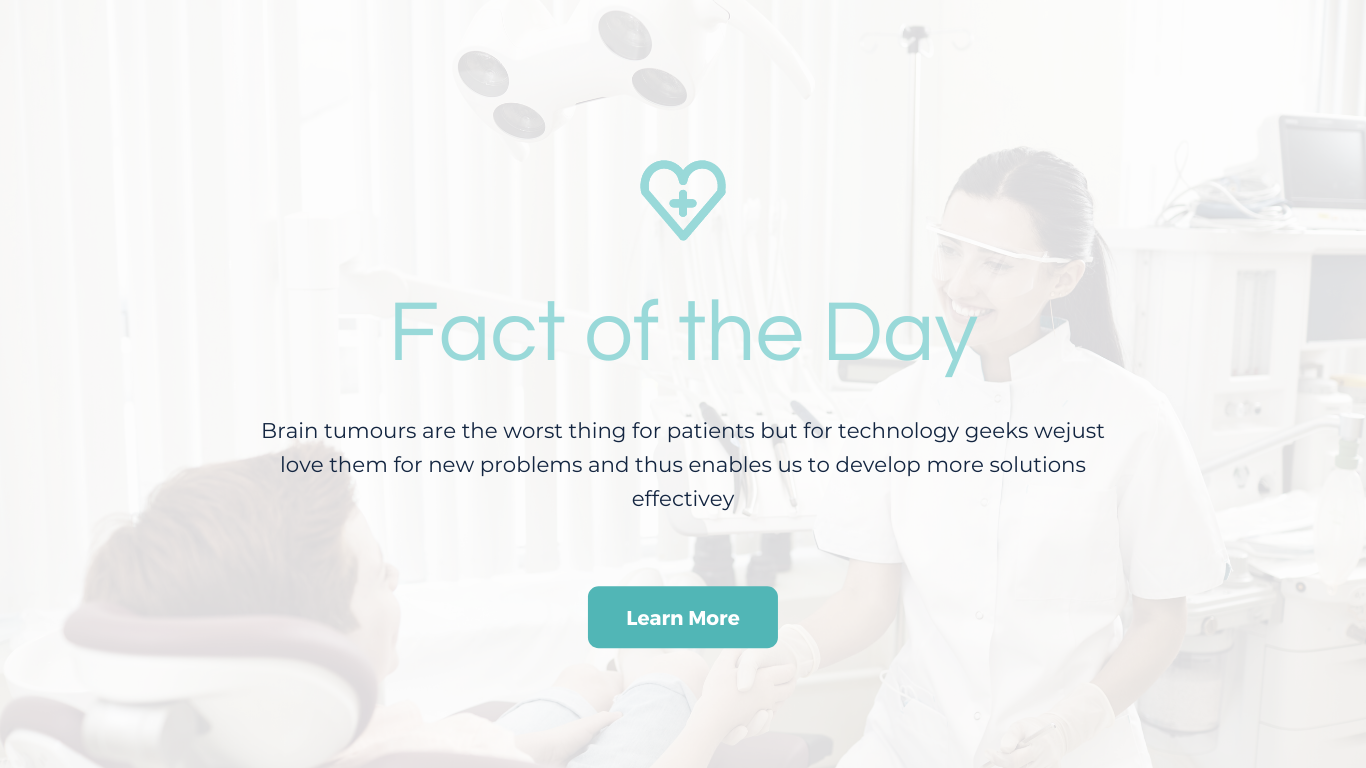
\includegraphics[scale=0.45]{Photos/webapp_2.png}
\caption{Fact of the Day} \label{fig:webapp_2}
\end{figure}
The next figure(\ref{fig:webapp_3}) refers to the "Our Services" page. Here the patients will be able to access any previous history if any as well as perform the actual Brain Tumor Detection. The traditional procedures tab will highlight about the traditional existing methods that are used in the detection procedure.
\begin{figure}[H]
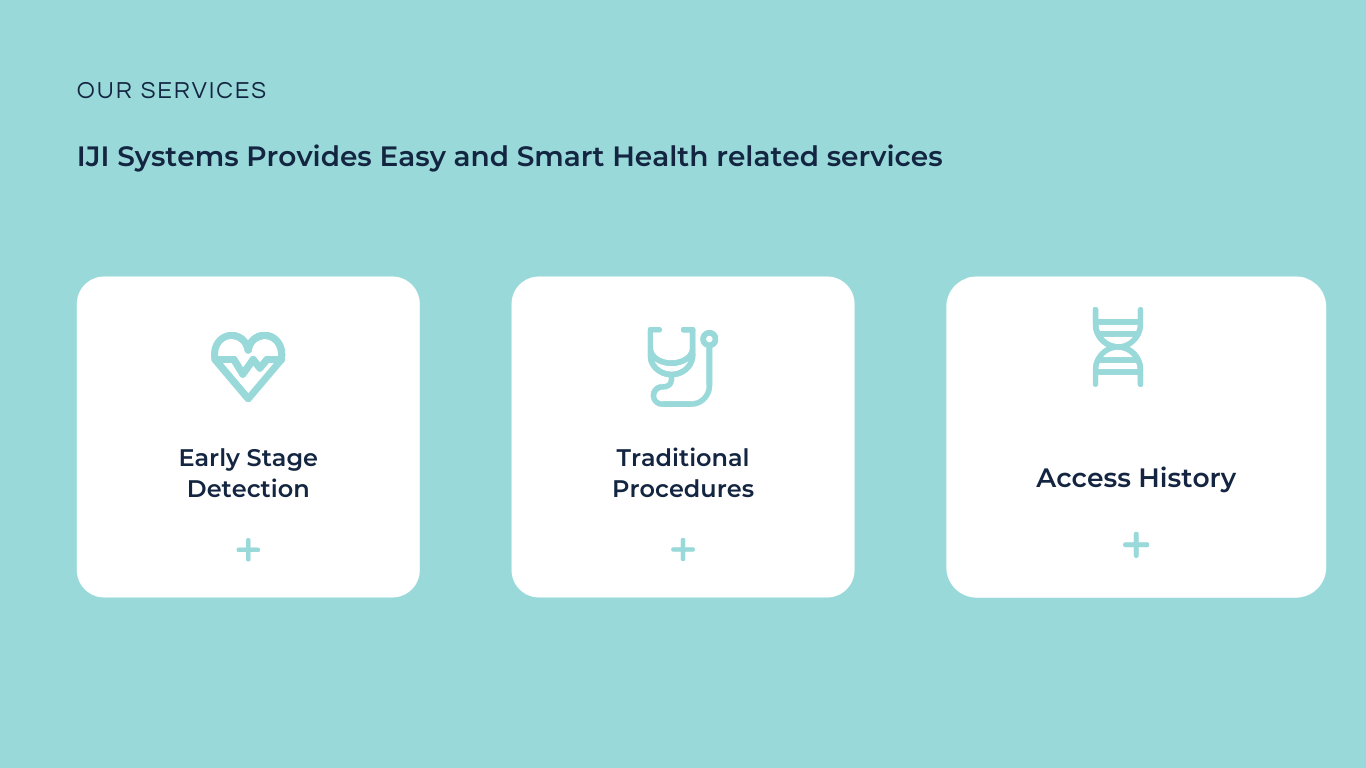
\includegraphics[scale=0.45]{Photos/webapp_3.png}
\caption{Page to Redirect to different functionalities} \label{fig:webapp_3}
\end{figure}
The figure \ref{fig:webapp_4} is the proposed Detection page. Here users will be able to upload the scanned MRI images. The system will then determine about Tumor and provide the results accordingly.
\begin{figure}[H]
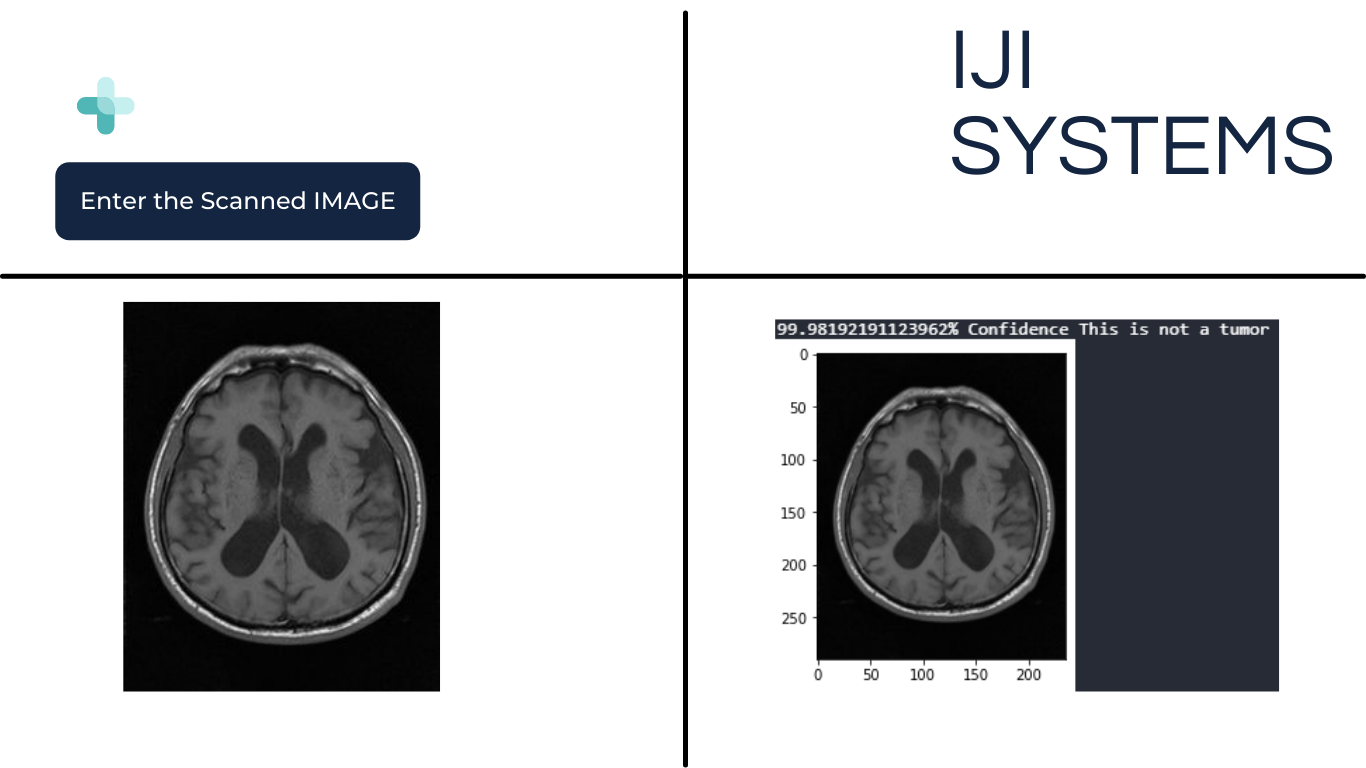
\includegraphics[scale=0.45]{Photos/webapp_4.png}
\caption{Brain Tumor Detection} \label{fig:webapp_4}
\end{figure}
Figure \ref{fig:webapp_5} highlights the team information page.
\begin{figure}[H]
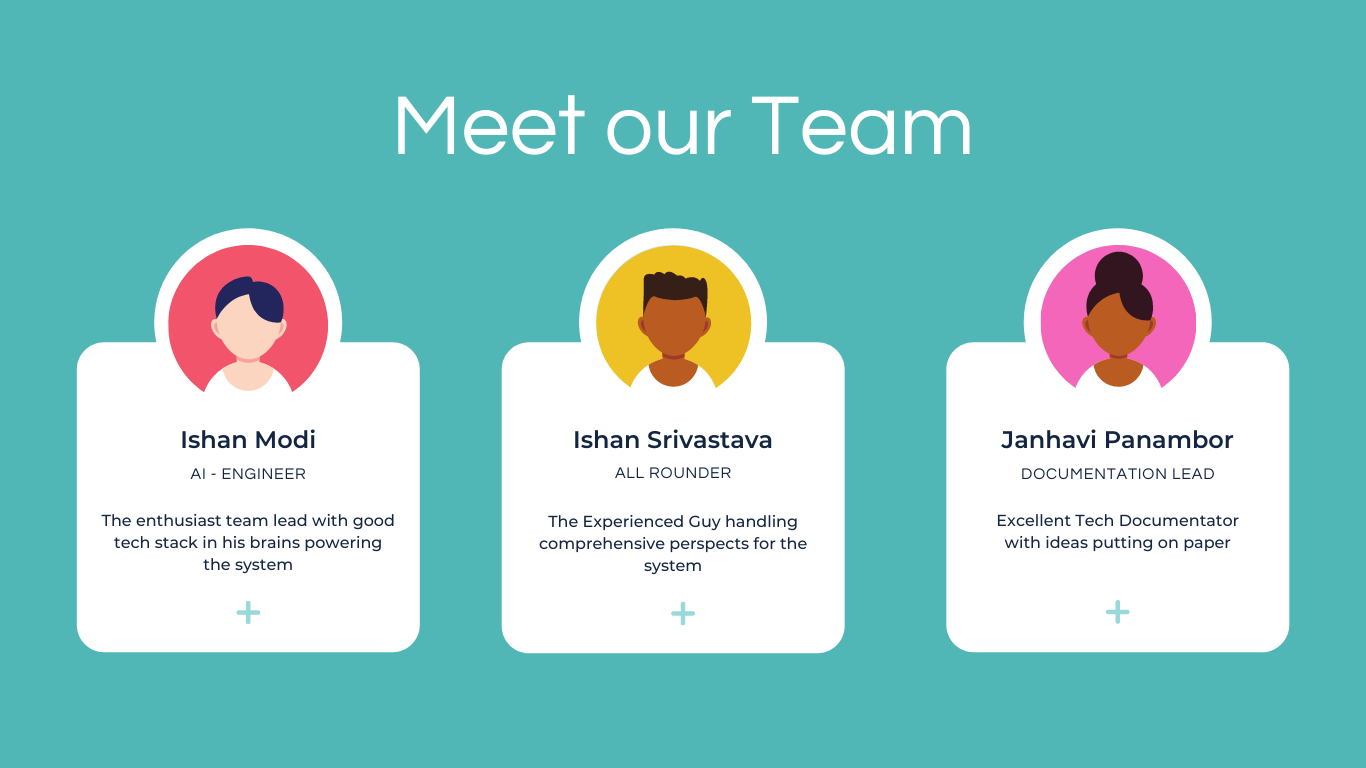
\includegraphics[scale=0.45]{Photos/webapp_5.png}
\caption{Team Information Page} \label{fig:webapp_5}
\end{figure}
Figure \ref{fig:webapp_6} highlights the Contact Us page.
\begin{figure}[H]

\includegraphics[scale=0.45]{Photos/webapp_6.png}
\caption{Contact Us Page} \label{fig:webapp_6}
\end{figure}
\chapter{Results and Discussion}
For the development phase of the project 2 Datasets have been used for training namely: 
\begin{itemize}
    \item \href{https://www.kaggle.com/navoneel/brain-mri-images-for-brain-tumor-detection}{Brain MRI Images for Brain Tumor Detection}
    \item \href{https://www.kaggle.com/ahmedhamada0/brain-tumor-detection}{Br35H :: Brain Tumor Detection 2020}
\end{itemize}
However Dataset 1 is a small dataset, there were not enough examples to train the neural network. Hence Data augmentation, was performed on Dataset 1. Data augmentation also is useful in taclking the data imbalance issue in the data. With this updated Dataset we merged both of these Datasets(Augmented dataset1 and dataset2) into a single final dataset. All this data was then passed onto a final dataset, which was then separated into 3 segments: Train , Test and Validation in ratio of 70:15:15. Then these train images were passed on to the model. The model then was trained for 6 times. Each version trained had a different parameter associated with it. These parameters and results associated with each result can be understood in the section \ref{section:results}.
Based on the results from each verion the highest accuracy achieved is 100\%. However the loss associated with that version suggests overfitting. Overfitting according to \href{https://en.wikipedia.org/wiki/Overfitting}{Wikipedia} is "the production of an analysis that corresponds too closely or exactly to a particular set of data, and may therefore fail to fit additional data or predict future observations reliably".Hence, the next best version with an accuracy of 92\% is taken into consideration for further development. This final model was then manually tested with a \href{https://www.kaggle.com/preetviradiya/brian-tumor-dataset}{third dataset}, to test the accuracy of the model. The Model is efficiently able to classify MRI Scan into Tumorous and Non Tumorous Image Respectively.

\section{Dataset Information}
Table \ref{tab:bef_aug} displays the number of imgaes in each dataset before augmentation\\
\begin{table}[h!]
\caption{Contents of dataset before augmentation}
\label{tab:bef_aug}
\begin{tabular}{|c|c|c|}
\hline
\rowcolor[HTML]{CBCEFB} 
\textbf{Dataset} & \textbf{Tumorous Images} & \textbf{Non Tumorous Images} \\ \hline
Dataset 1        & 155                      & 98                           \\ \hline
Dataset 2        & 1500                     & 1500                         \\ \hline
Dataset 3        & 2513                     & 2087                         \\ \hline
\end{tabular}
\end{table}

\noindent Table \ref{tab:af_aug} displays the number of imgaes in each dataset after augmentation\\
\begin{table}[h!]
\caption{Contents of dataset after augmentation}
\label{tab:af_aug}
\begin{tabular}{|c|c|c|}
\hline
\rowcolor[HTML]{CBCEFB} 
\textbf{Dataset} & \textbf{Tumorous Images} & \textbf{Non Tumorous Images} \\ \hline
Dataset 1        & 1083                      & 980                           \\ \hline
Dataset 2        & 1500                     & 1500                         \\ \hline
Dataset 3        & 2513                     & 2087                         \\ \hline
\end{tabular}
\end{table}

\noindent Table \ref{tab:final_data} displays the number of imgaes in the final dataset after merging\\
\begin{table}[h!]
\caption{Contents of final dataset}
\label{tab:final_data}
\begin{tabular}{|c|c|c|}
\hline
\rowcolor[HTML]{CBCEFB} 
\textbf{Dataset} & \textbf{Tumorous Images} & \textbf{Non Tumorous Images} \\ \hline
Final Dataset    & 2583                     & 2480                         \\ \hline
\end{tabular}
\end{table}

\section{Training Results}
\label{section:results}
As part of model training different approaches were considered. Some of the main parameters into consideration are as follows:
\begin{itemize}
    \item Amount of images used.
    \item Transfer learning.
    \item Creating callbacks to prevent overtraining.
\end{itemize}
Table \ref{tab:result} highlights the different results obtained with each version alongwith the parameter changes performed.\\
% Please add the following required packages to your document preamble:
% \usepackage{multirow}
% \usepackage{graphicx}
% \usepackage[table,xcdraw]{xcolor}
% If you use beamer only pass "xcolor=table" option, i.e. \documentclass[xcolor=table]{beamer}
% Please add the following required packages to your document preamble:
% \usepackage{multirow}
% \usepackage{graphicx}
% \usepackage[table,xcdraw]{xcolor}
% If you use beamer only pass "xcolor=table" option, i.e. \documentclass[xcolor=table]{beamer}
% Please add the following required packages to your document preamble:
% \usepackage{multirow}
% \usepackage{graphicx}
% \usepackage[table,xcdraw]{xcolor}
% If you use beamer only pass "xcolor=table" option, i.e. \documentclass[xcolor=table]{beamer}
\begin{table}[h!]
\caption{Results obtained from each version}
\label{tab:result}
\resizebox{\textwidth}{!}{%
\begin{tabular}{|c|cc|c|c|c|c|c|}
\hline
\rowcolor[HTML]{CBCEFB} 
\cellcolor[HTML]{CBCEFB}                             & \multicolumn{2}{c|}{\cellcolor[HTML]{CBCEFB}Number of Images Used}   & \cellcolor[HTML]{CBCEFB}                                                                       & \cellcolor[HTML]{CBCEFB}                                                                                         & \cellcolor[HTML]{CBCEFB}                            & \cellcolor[HTML]{CBCEFB}                                & \cellcolor[HTML]{CBCEFB}                                                                                                                                                                             \\ \cline{2-3}
\rowcolor[HTML]{CBCEFB} 
\multirow{-2}{*}{\cellcolor[HTML]{CBCEFB}Version \#} & \multicolumn{1}{c|}{\cellcolor[HTML]{CBCEFB}Tumorous} & Non-Tumorous & \multirow{-2}{*}{\cellcolor[HTML]{CBCEFB}\begin{tabular}[c]{@{}c@{}}Model\\ Type\end{tabular}} & \multirow{-2}{*}{\cellcolor[HTML]{CBCEFB}\begin{tabular}[c]{@{}c@{}}No. of Datasets \\ Implemented\end{tabular}} & \multirow{-2}{*}{\cellcolor[HTML]{CBCEFB}Test Loss} & \multirow{-2}{*}{\cellcolor[HTML]{CBCEFB}Test Accuracy} & \multirow{-2}{*}{\cellcolor[HTML]{CBCEFB}\begin{tabular}[c]{@{}c@{}}Additional Parameters/\\ Notes\end{tabular}}                                                                                     \\ \hline
\#1                                                  & \multicolumn{1}{c|}{155}                              & 98           & \begin{tabular}[c]{@{}c@{}}CNN:\\ InceptionResNetV2\end{tabular}                               & 1(Dataset 1)                                                                                                     & 0.4165                                              & 0.7692                                                  & \begin{tabular}[c]{@{}c@{}}Transfer Learning on \\ InceptionResNetV2\end{tabular}                                                                                                                    \\ \hline
\#2                                                  & \multicolumn{1}{c|}{1083}                             & 980          & \begin{tabular}[c]{@{}c@{}}CNN:\\ InceptionResNetV2\end{tabular}                               & \begin{tabular}[c]{@{}c@{}}2(Dataset 1, and\\ Augmented)\end{tabular}                                            & 0.0351                                              & 1                                                       & \begin{tabular}[c]{@{}c@{}}1) Transfer Learning on \\ InceptionResNetV2\\ 2) Data imbalance resolved\\ 3)Overfitting observed. Huge gap\\ observed between Train and\\ Validation loss.\end{tabular} \\ \hline
\#3                                                  & \multicolumn{1}{c|}{155}                              & 98           & CNN : Custom                                                                                   & 1(Dataset 1)                                                                                                     & 0.8249                                              & 0.8571                                                  & \begin{tabular}[c]{@{}c@{}}1) Unbalanced Data\\ 2) Custom Model\end{tabular}                                                                                                                         \\ \hline
\#4                                                  & \multicolumn{1}{c|}{1083}                             & 980          & CNN : Custom                                                                                   & \begin{tabular}[c]{@{}c@{}}2(Dataset 1, and\\ Augmented)\end{tabular}                                            & 1.0134                                              & 0.7936                                                  & \begin{tabular}[c]{@{}c@{}}1) Data Imbalance Resolved\\ 2) Huge gap between Train and \\ Validation accuracy observed\end{tabular}                                                                   \\ \hline
\#5                                                  & \multicolumn{1}{c|}{1083}                             & 980          & CNN : Custom                                                                                   & \begin{tabular}[c]{@{}c@{}}2(Dataset 1, and\\ Augmented)\end{tabular}                                            & 0.9547                                              & 0.8281                                                  & Callbacks Defined                                                                                                                                                                                    \\ \hline
\#6                                                  & \multicolumn{1}{c|}{2583}                             & 2480         & CNN : Custom                                                                                   & \begin{tabular}[c]{@{}c@{}}3(Dataset 1,\\ Augmented and\\ Dataset 2)\end{tabular}                                & 0.3819                                              & 0.9206                                                  & Data Increased                                                                                                                                                                                       \\ \hline
\end{tabular}%
}
\end{table}

\noindent Figure \ref{fig:v1} - \ref{fig:v6} highlight the loss and accuracy graph of each version.\\
Version 1 implemented transfer learning on InceptionResNetV2. However
 the graphs of loss and accuracy for version 1 is not consistent for each epoch, indicating that the system when manually tested will have a higher chance of providing false results.
\begin{figure}[H]
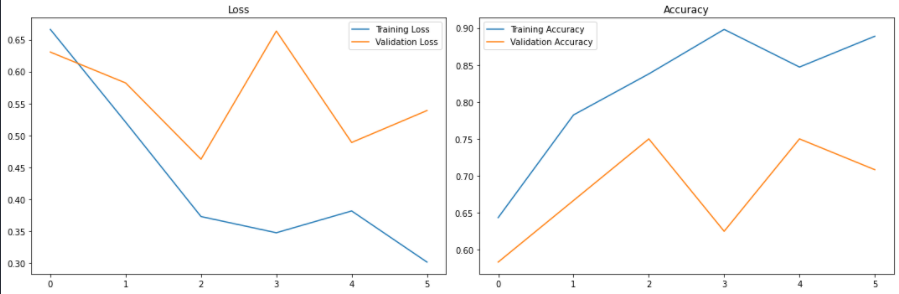
\includegraphics[scale=0.6]{Photos/v1.PNG}
\caption{Loss and Accuracy Graph of Version 1} \label{fig:v1}
\end{figure}

Version 2 is a successor to version 1. Augmented data was used for training here. This version provides the best accuracy compared to other versions. However on seeing the loss graph it can be observed that there is a huge gap between train and validation loss indicating overfitting.
\begin{figure}[H]
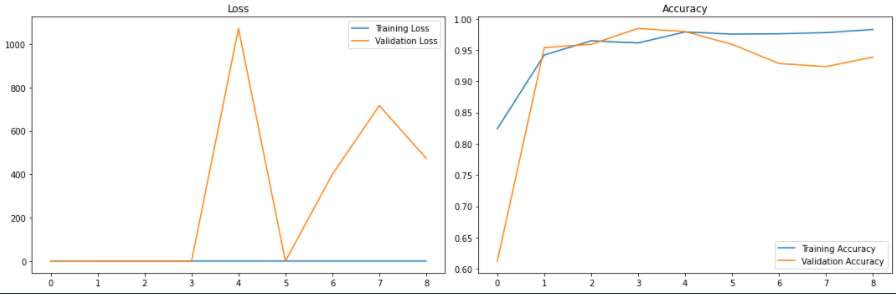
\includegraphics[scale=0.6]{Photos/v2.PNG}
\caption{Loss and Accuracy Graph of Version 2} \label{fig:v2}
\end{figure}

Version 3 implemented a custom CNN model architecture. However the amount of images used were less, leading to a higher test loss and lower test accuracy.
\begin{figure}[H]
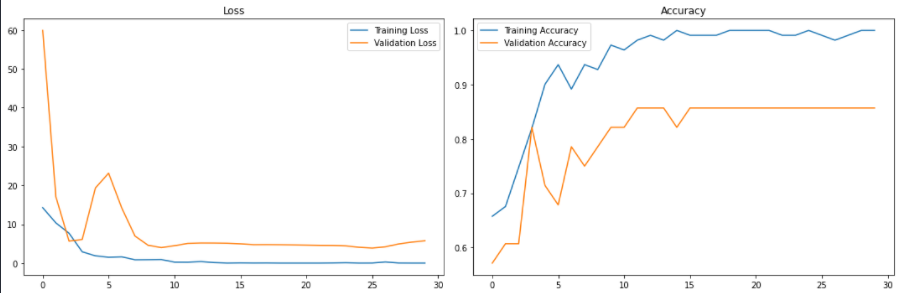
\includegraphics[scale=0.6]{Photos/v3.PNG}
\caption{Loss and Accuracy Graph of Version 3} \label{fig:v3}
\end{figure}

Version 4 uses augmented data to try and resolve the issues faced from version 3. However on seeing the graphs it can be inferred that the model is overfitting.
\begin{figure}[H]
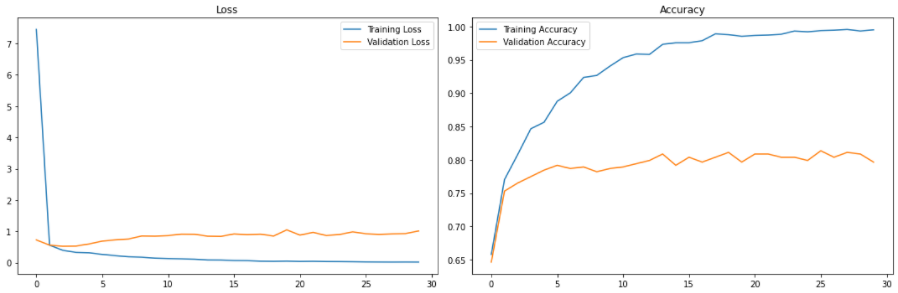
\includegraphics[scale=0.6]{Photos/v4.PNG}
\caption{Loss and Accuracy Graph of Version 4} \label{fig:v4}
\end{figure}

Version 5 implements usage of callbacks to reduce this overfitting issue. The callbacks implemented are:
\begin{itemize}
    \item EarlyStopping : Early stopping is a method that allows user to specify an arbitrary large number of training epochs and stop training once the model performance stops improving on a hold out validation dataset.
    \item ModelCheckpoint : ModelCheckpoint is used to save a model or weights (in a checkpoint file) at some interval, so the model or weights can be loaded later to continue the training from the state saved.
\end{itemize}
Using callbacks test loss decreased, and test accuracy increased to an extent.
\begin{figure}[H]
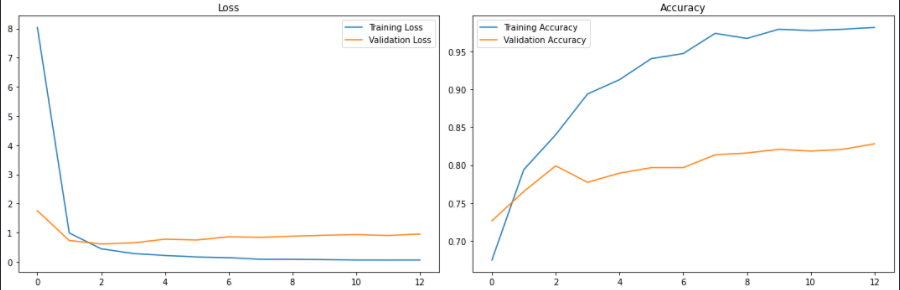
\includegraphics[scale=0.6]{Photos/v5.PNG}
\caption{Loss and Accuracy Graph of Version 5} \label{fig:v5}
\end{figure}

To further improve the results obtained from version 5, volume of images used was increased, leading to the best performing model compared to the previous ones.
\begin{figure}[H]
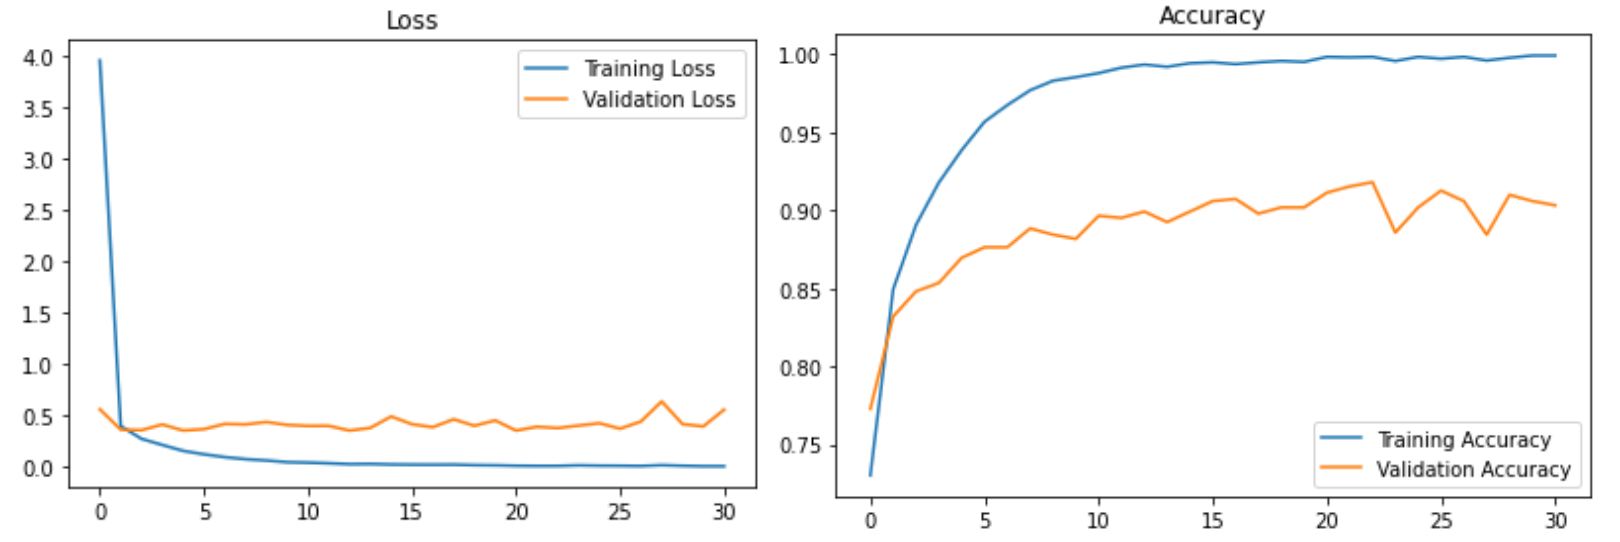
\includegraphics[scale=0.35]{Photos/v6.png}
\caption{Loss and Accuracy Graph of Version 6} \label{fig:v6}
\end{figure}
    
\section{Manual Test Results}
In Manual Testing images from the third dataset were used to test the model on individual images. The images from third dataset have not been used to training of the model at any point; hence it acts as unbiased data. The results from the manual testing are as follows:
\begin{itemize}
    \item Tumour Present in the Brain:
        \begin{figure}[H]
        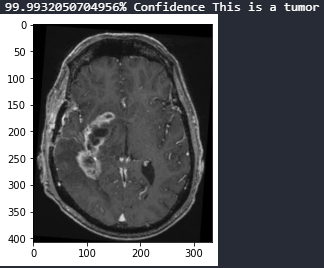
\includegraphics[scale=0.8]{Photos/Tumor_Manual_Result.PNG}
        \caption{Tumour Manual Testing Results} \label{fig:ishan}
        \end{figure}
    \item Tumour Absent in the Brain:
        \begin{figure}[H]
        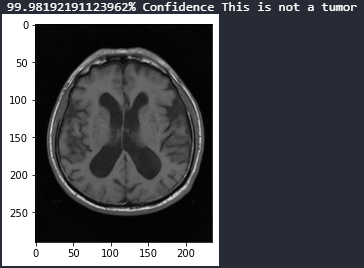
\includegraphics[scale=0.8]{Photos/Non_Tumor_Manual_Result.PNG}
        \caption{Non-Tumour Manual Testing Results} \label{fig:ishan}
        \end{figure}
\end{itemize}
\chapter{Conclusions and Future Scope}
\section{Conclusions }
Implementation of a Deep Learning Model which detects whether there is brain tumour present or not is observed. A total of 6 versions based on CNN are developed with various parameters into consideration. Based on these results and further testing the model with the best accuracy gives an system accuracy of 92\%. This result is verified using model evaluate function as well as the manual image set testing. Input image is passed onto the trained model which then determines whether image contains tumour or not. As per the inference by the model the output will be displayed on the web application accordingly.
\section{Future Scope }
\begin{itemize}
    \item The particular trained model can be further trained to detect tumour of initial stages.
    \item The particular model can be trained further to detect which type of brain tumour is present inside the body.
    \item The system in it’s base form can be trained further to detect the tumour even more efficiently
    \item The entire Web Application can be further developed to understand more types of human body scans such as X-ray, CT - Scans etc. So as to become a full fledged health assessment portal.
    \item Such web application could be installed at hospitals which will then connect patients and the hospital staff virtually.
    \item The system can be upgraded to detect more types of tumours such as ovarian, breast, skin, lung tumours etc.
\end{itemize}


\addcontentsline{toc}{chapter}{References}
\renewcommand\bibname{References}
\begin{thebibliography}{99}
\bibitem{ref1}Avigyan Sinha, Aneesh R P, Malavika Suresh, Nitha Mohan R, Abinaya D, Ashwin G Singerji ``Brain Tumour Detection Using Deep Learning`` \textit{Seventh International conference on Bio Signals, Images, and Instrumentation (ICBSII)}, 2021

\bibitem{ref2}Pär Salander, A Tommy Bergenheim, Katarina Hamberg, Roger Henriksson , ``Pathways from symptoms to medical care: a descriptive study of symptom development and obstacles to early diagnosis in brain tumour patients`` \textit{Family Practice, Volume 16, Issue 2, April 1999, Pages 143–148}

\bibitem{ref3}McKinney PA, ``Brain tumours: incidence, survival, and aetiology,`` \textit{Journal of Neurology, Neurosurgery \& Psychiatry 2004}

\bibitem{ref4}Muhammad Waqas Nadeem, Mohammed A. Al Ghamdi, Muzammil Hussain, Muhammad Adnan Khan, Khalid Masood Khan, Sultan H. Almotiri and Suhail Ashfaq Butt, ``Brain Tumor Analysis Empowered with Deep Learning: A Review, Taxonomy, and Future Challenges`` \textit{Brain Sci.}2020

\bibitem{ref5}Logeswari, T.; Karnan, M.``An improved implementation of brain tumor detection using segmentation based on hierarchical self organizing map.`` \textit{Int. J. Comput. Theory Eng. 2010, 2, 591.}

\bibitem{ref6}Yang, G.; Raschke, F.; Barrick, T.R.; Howe, F.A.``Manifold Learning in MR spectroscopy using nonlinear dimensionality reduction and unsupervised clustering.`` \textit{Magn. Reson. Med. 2015, 74, 868–878. }

\bibitem{ref7}Mansi Lathera, Dr. Parvinder Singh``Investigating Brain Tumor Segmentation and Detection Techniques `` \textit{International Conference on Computational Intelligence and Data Science (ICCIDS 2019)}

\bibitem{ref8}Nandita Goyal and Dr. Bharti Sharma``Image Processing Techniques for Brain Tumor Identification`` \textit{IOP Conf. Ser.: Mater. Sci. Eng. 1022 012011}

\bibitem{ref9}Isselmou Abd El Kader, Guizhi Xu, Zhang Shuai, Sani Saminu, Imran Javaid, Isah Salim Ahmad and Souha Kamhi``Brain Tumor Detection and Classification on MR Images by a Deep Wavelet Auto-Encoder Model`` \textit{Diagnostics 2021}

\bibitem{ref10}Saurabh Kumar, Iram Abid, Shubhi Garg, Anand Kumar Singh and Vivek Jain``BRAIN TUMOR DETECTION USING IMAGE PROCESSING`` \textit{International Journal of Information Sciences and Application (IJISA). ISSN 0974-2255, Vol.11, No.1, 2019, (Special Issue)}

\bibitem{ref11}Ramin Ranjbarzadeh, Abbas Bagherian Kasgari, Saeid JafarzadehGhoushchi, ShokofehAnari, Maryam Naseri \& Malika Bendechache``Brain tumor segmentation based on deep learning and an attention mechanism using MRI multi‑modalities brain images``
\end{thebibliography}
\end{document}
